\documentclass[11pt,a4paper]{article}
\usepackage[margin=27mm,headheight=15pt]{geometry}
\usepackage[T1]{fontenc}
\usepackage[utf8]{inputenc}
\IfFileExists{libertinus.sty}{\usepackage{libertinus}}{\usepackage{lmodern}}
\usepackage{microtype,amsmath,amssymb,amsthm,mathtools,mathrsfs}
\usepackage{booktabs,longtable,array,graphicx,xcolor,fancyhdr}
\usepackage{xurl}
\usepackage[hypertexnames=false]{hyperref}
\hypersetup{colorlinks=true,linkcolor=blue!45!black,citecolor=blue!45!black,urlcolor=blue!45!black,
 pdftitle={A Dyadic Completion of the Thue--Morse Product},
 pdfauthor={Research article prepared for Vladimir Reshetnikov},
 pdfsubject={Mellin transforms, horizontal zero strings, lognormal moments, certified asymptotics}}
\usepackage{aliascnt}
\usepackage[nameinlink,noabbrev]{cleveref}
\usepackage{listings}
\lstset{basicstyle=\ttfamily\small,breaklines=true,columns=fullflexible,frame=single}
\pagestyle{fancy}\fancyhf{}
\fancyhead[L]{\small Thue--Morse: dyadic completion}
\fancyhead[R]{\small Mellin transforms and zero asymptotics}
\fancyfoot[C]{\thepage}
\setlength{\emergencystretch}{3em}
\allowdisplaybreaks
\numberwithin{equation}{section}
\newtheorem{theorem}{Theorem}[section]
\newaliascnt{lemma}{theorem}
\newtheorem{lemma}[lemma]{Lemma}
\aliascntresetthe{lemma}
\crefname{lemma}{lemma}{lemmas}
\Crefname{lemma}{Lemma}{Lemmas}
\newaliascnt{proposition}{theorem}
\newtheorem{proposition}[proposition]{Proposition}
\aliascntresetthe{proposition}
\crefname{proposition}{proposition}{propositions}
\Crefname{proposition}{Proposition}{Propositions}
\newaliascnt{corollary}{theorem}
\newtheorem{corollary}[corollary]{Corollary}
\aliascntresetthe{corollary}
\crefname{corollary}{corollary}{corollaries}
\Crefname{corollary}{Corollary}{Corollaries}
\theoremstyle{definition}
\newaliascnt{definition}{theorem}
\newtheorem{definition}[definition]{Definition}
\aliascntresetthe{definition}
\crefname{definition}{definition}{definitions}
\Crefname{definition}{Definition}{Definitions}
\newaliascnt{example}{theorem}
\newtheorem{example}[example]{Example}
\aliascntresetthe{example}
\crefname{example}{example}{examples}
\Crefname{example}{Example}{Examples}
\theoremstyle{remark}
\newaliascnt{remark}{theorem}
\newtheorem{remark}[remark]{Remark}
\aliascntresetthe{remark}
\crefname{remark}{remark}{remarks}
\Crefname{remark}{Remark}{Remarks}
\newaliascnt{question}{theorem}
\newtheorem{question}[question]{Question}
\aliascntresetthe{question}
\crefname{question}{question}{questions}
\Crefname{question}{Question}{Questions}
\newcommand{\eps}{\varepsilon}
\newcommand{\E}{\mathbb E}
\newcommand{\R}{\mathbb R}
\newcommand{\C}{\mathbb C}
\newcommand{\Z}{\mathbb Z}
\newcommand{\N}{\mathbb N}
\newcommand{\ii}{\mathrm i}
\newcommand{\dd}{\,\mathrm d}
\DeclareMathOperator{\Log}{Log}
\newcommand{\Rea}{\operatorname{Re}}
\newcommand{\Ima}{\operatorname{Im}}
\newcommand{\coef}[2]{[#1^{#2}]}
\newcommand{\qbinom}[3]{\genfrac{[}{]}{0pt}{}{#1}{#2}_{#3}}
\newcommand{\abs}[1]{\left|#1\right|}
\newcommand{\calH}{\mathcal H}
\newcommand{\sourcepath}{\path{Analysis/FabiusFunction/docs/semi-formalized-research-frontiers/drafts/thue-morse/Thue_Morse_Atlas_and_Frontiers/Thue_Morse_Atlas_and_Frontiers.tex}}

\title{\bfseries A Dyadic Completion of the Thue--Morse Product\\[0.4em]
\Large Lognormal moments, horizontal Dirichlet zero strings,\\
and certified all-orders asymptotics}
\author{Research article prepared for Vladimir Reshetnikov\\
\small An extension of the \texttt{ProveIt} Thue--Morse atlas}
\date{4 September 2026}

\begin{document}
\maketitle
\begin{abstract}
The familiar Thue--Morse product
$P(t)=\prod_{j\ge0}(1-e^{-2^jt})$ has a particularly useful completion.
If $X=\sum_{j\ge1}2^{-j}U_j$, with independent uniform $U_j$ on $[0,1]$,
and $\Phi(t)=\E e^{-tX}$, then $K(t)=P(t)\Phi(t)$ satisfies exactly
$K(2t)=K(t)/t$. Its Mellin transform $C(s)$ therefore satisfies
$C(s+1)=2^{s+1}C(s)$. The resulting positive density has all integer
moments of a lognormal distribution, but is not lognormal.

The central application concerns the entire continuation of
$D(s,a)=\sum_{n\ge0}(-1)^{s_2(n)}(n+a)^{-s}$, for $a>0$.
We prove a locally uniform all-orders scaling formula for
$\Gamma(s-m)D(s-m,a)$. Its limiting function is $C(s)$, and every
coefficient is an explicit polynomial-exponential multiple of $C(s)$.
A nonconstant, entire, finite-order periodic factor of $C$ must have
nonreal zeros. Rouch\'e's theorem transfers each such zero $s_0$ to
zeros of $D(s,a)$ near $s_0-m$, with errors smaller than $2^{-Am}$
for every fixed $A>0$. Thus every positive shift has infinitely many
nonreal zeros in the left half-plane. For the half-shift, the error
can be bounded on a Gaussian scale in $m$.

We also derive finite coefficient formulas for the derivatives at the
real zeros. At the centered shift $a=1/2$, their normalized values
are samples of one completely monotone function. Its divergent
expansion has an alternating remainder bounded by its first omitted
term at every order. Explicit coefficient asymptotics give an
optimized error of size $\exp[-(\log2)m^2/2+O(m)]$.
The proofs, numerical checks, and a careful distinction between
classical ingredients and research extensions are supplied in full.
\end{abstract}
\begingroup\small
\tableofcontents
\endgroup
\clearpage

\section{Scope, provenance, and principal conclusions}
\label{sec:scope}

\subsection{What is being extended}
The source atlas \cite{atlas} already develops the binary recurrences,
Prouhet cancellation, dyadic finite products, power moments, Fourier
representations, rarefied sums, and the Mellin continuation of the
Thue--Morse Dirichlet family. Repeating those chapters would not be a
useful extension. This article instead connects three pieces of that
framework: the lacunary Laplace product, the compactly supported
uniform-convolution law underlying the Fabius function, and the
Dirichlet continuation at large negative arguments.

The notation is independent of the repository's macro files, so this
source compiles without a checkout of the repository. We write
\begin{equation}
 \eps_n=(-1)^{s_2(n)},\qquad L=\log2,
 \qquad D(s,a)=\sum_{n\ge0}\frac{\eps_n}{(n+a)^s}.
 \label{eq:notation}
\end{equation}
Here $s_2(n)$ is the number of $1$'s in the binary expansion of $n$.
The shift $a$ is always a positive real number unless explicitly stated
otherwise. A prime on $D$ means differentiation with respect to $s$.
The Mellin transform uses the measure $t^{s-1}\dd t$.

\subsection{Research status and attribution}
Entireness of the Thue--Morse Dirichlet continuation is classical:
see Allouche--Cohen \cite{AC}, the general automatic-series theory
\cite{AMP}, and the subsequent treatment \cite{Toth}. The uniform
series and its Fabius connection are also established background
\cite{Arias,Haugland,atlas}. Lognormal moment indeterminacy,
size-bias scaling, and geometric-lattice representations are classical
\cite{AGK}. None of those subjects is claimed as newly discovered here.

The principal research contribution of the present derivation is the
\emph{combined} completion--Mellin--zero mechanism, together with the
coefficientwise factorization of the scaled Dirichlet expansion and
the global signed remainder theorem at the half-shift. These are
proved below, not merely suggested by experiments. Their mathematical
validity and their bibliographical priority are separate questions.
The literature search did not establish priority, and one relevant
2001 preprint by Alkauskas \cite{Alkauskas} could not be retrieved.
Consequently ``proved here'' never means ``proved here for the first
time in the literature.'' A more detailed audit is in
\cref{sec:audit}.

The zero theorem has a specific historical consequence. Section 3.2
of Allouche's survey \cite{AlloucheQuestions} asks whether the
nontrivial zeros of $D(s,1)$ consist only of
$2\pi\ii k/L$. The theorem below supplies zeros with negative real
part, and hence a negative answer to that exact question. This is a
consequence of the proof, not a claim that the question has remained
unresolved until the date of this article.

\subsection{The main theorem in one place}
Define
\begin{equation}
 P(t)=\prod_{j\ge0}(1-e^{-2^jt}),\qquad
 \Phi(t)=\prod_{j\ge1}\frac{1-e^{-t/2^j}}{t/2^j},
 \qquad K(t)=P(t)\Phi(t).
 \label{eq:three-products}
\end{equation}
For $t>0$ all three functions are positive. Put
\begin{equation}
 C(s)=\int_0^\infty t^{s-1}K(t)\dd t,
 \qquad C_0=C(0),\qquad
 Q(s)=\frac{C(s)}{C_0\,2^{s(s+1)/2}}.
 \label{eq:CQ-def}
\end{equation}
The powers of $2$ always mean $e^{Lz}$, with no branch choice.

\begin{theorem}[Completion and horizontal zero strings]
\label{thm:overview}
The integral $C(s)$ is entire; $Q$ is entire, $1$-periodic,
positive on the real axis, nonconstant, and of order at most two.
In particular, $C$ has a nonreal zero.

If $s_0$ is any zero of $C$ of multiplicity $d$, then for each fixed
$a>0$ and all sufficiently large integers $m$, $D(\cdot,a)$ has a
cluster of $d$ zeros near $s_0-m$. For every $A>0$ these zeros lie in
\begin{equation}
 \abs{s-(s_0-m)}<2^{-Am}
 \label{eq:zero-supergeometric}
\end{equation}
for all sufficiently large $m$ depending on $A,a,s_0$.
The clusters for different sufficiently large $m$ are disjoint.
For $a=1/2$, the stronger bound
\begin{equation}
 \abs{s-(s_0-m)}\le
 \exp\left(-\frac{L}{2d}m^2+O_{s_0}(m)\right)
 \label{eq:zero-gaussian}
\end{equation}
holds. Every $a>0$ therefore has infinitely many nonreal zeros in the
left half-plane, including the unshifted-denominator case $a=1$.
\end{theorem}

The ingredients and proof of the first bound occupy
\cref{sec:completion,sec:mellin,sec:dirichlet,sec:scaling,sec:zeros}.
The quantitative refinement is proved in \cref{sec:complex-center}.
The use of ``cluster'' allows multiple zeros of $C$; simplicity is not
assumed. No numerical zero enclosure is needed for the theorem.

\section{From binary cancellation to a completed product}
\label{sec:completion}

\subsection{The elementary finite product}
The binary identities
\begin{equation}
 \eps_{2n}=\eps_n,\qquad \eps_{2n+1}=-\eps_n
 \label{eq:binary}
\end{equation}
give, by expanding one factor for each binary digit,
\begin{equation}
 \sum_{n=0}^{2^m-1}\eps_n z^n
 =\prod_{j=0}^{m-1}(1-z^{2^j}).
 \label{eq:finite-product}
\end{equation}
For $\abs z<1$, both sides tend to
$\sum_{n\ge0}\eps_nz^n=\prod_{j\ge0}(1-z^{2^j})$.
The products converge normally on compact subsets of the unit disk
because $\sum_j\abs z^{2^j}<\infty$ there. In particular,
\begin{equation}
 P(t)=\sum_{n\ge0}\eps_n e^{-nt},\qquad
 P(2t)=\frac{P(t)}{1-e^{-t}}
 \quad(t>0).
 \label{eq:P-mahler}
\end{equation}
The same product defines a holomorphic function for $\Rea t>0$.

For each integer $r\ge0$, using the first $r$ factors and bounding the
others by one gives
\begin{equation}
 0<P(t)\le 2^{r(r-1)/2}t^r.
 \label{eq:flat-bound}
\end{equation}
Thus $P$ is smaller than every fixed power at the origin. This
cancellation is the analytic counterpart of the vanishing of the
first $m$ power moments in \cref{eq:finite-product}.

\subsection{The compact uniform series}
Let $U_1,U_2,\ldots$ be independent random variables uniformly
distributed on $[0,1]$, and define
\begin{equation}
 X=\sum_{j=1}^\infty 2^{-j}U_j.
 \label{eq:X}
\end{equation}
The series converges surely, and $0\le X\le1$. Independence and
bounded convergence give the entire Laplace transform
\begin{equation}
 \Phi(z)=\E e^{-zX}
 =\prod_{j\ge1}\frac{1-e^{-z/2^j}}{z/2^j}.
 \label{eq:Phi-probability}
\end{equation}
Each factor is interpreted by continuity at $z=0$. Normal convergence
on compact sets follows either from its expansion $1-z/2^{j+1}+O(4^{-j})$
or from boundedness of $X$. The distribution is symmetric about
$1/2$, because replacing every $U_j$ by $1-U_j$ changes $X$ to $1-X$.
Furthermore,
\begin{equation}
 \E X=\frac12,\qquad
 \operatorname{Var}(X)=\frac1{12}\sum_{j\ge1}4^{-j}=\frac1{36}.
 \label{eq:X-moments}
\end{equation}
The density of $X$, or a linearly rescaled version of it, is one of
the standard uniform-convolution descriptions of the Fabius--Rvachev
family. Using $X$ avoids any ambiguity between conventions for those
functions.

Separating the first factor in \cref{eq:Phi-probability} gives
\begin{equation}
 \Phi(2t)=\frac{1-e^{-t}}{t}\Phi(t).
 \label{eq:Phi-dilation}
\end{equation}
This factor is exactly the inverse of the nonmonomial factor in the
scaling equation for $P$.

\begin{theorem}[Exact dyadic completion]
\label{thm:completion}
For every $t>0$,
\begin{equation}
 \boxed{K(2t)=\frac{K(t)}t.}
 \label{eq:K-dilation}
\end{equation}
For every integer $k$, positive or negative,
\begin{equation}
 K(2^kt)=2^{-k(k-1)/2}t^{-k}K(t).
 \label{eq:K-iterate}
\end{equation}
There is a positive, real-analytic, $L$-periodic function $H$ such that
\begin{equation}
 \boxed{K(t)=t^{1/2}
  \exp\left(-\frac{(\log t)^2}{2L}\right)H(\log t).}
 \label{eq:K-profile}
\end{equation}
In particular, constants $0<h_-\le h_+<\infty$ exist with
\begin{equation}
 h_-t^{1/2}e^{-(\log t)^2/(2L)}
 \le K(t)\le
 h_+t^{1/2}e^{-(\log t)^2/(2L)}.
 \label{eq:K-bounds}
\end{equation}
\end{theorem}
\begin{proof}
Multiply \cref{eq:P-mahler} and \cref{eq:Phi-dilation} to obtain
\cref{eq:K-dilation}. Induction upward and downward proves
\cref{eq:K-iterate}. Set
\[
 H(v)=e^{v^2/(2L)-v/2}K(e^v).
\]
Since $K(e^{v+L})=e^{-v}K(e^v)$, direct substitution shows
$H(v+L)=H(v)$. Positivity and continuity on $[0,L]$ give the two
positive bounds. Holomorphy of $K(e^v)$ in $\abs{\Ima v}<\pi/2$
gives real analyticity. The displayed representation and estimates
are now identities and consequences of compactness, respectively.
\end{proof}

\subsection{The periodic factor is genuinely present}
It is tempting to omit $H$, because its oscillation is numerically
small. Doing so would destroy the zero theorem and would replace the
actual moment measure by its lognormal twin.

\begin{proposition}[Nonconstancy]
\label{prop:H-nonconstant}
The function $H$ in \cref{eq:K-profile} is not constant.
\end{proposition}
\begin{proof}
Suppose that $H\equiv c>0$. Both $K(z)$ and
\[
 c\,z^{1/2}\exp\left(-\frac{(\Log z)^2}{2L}\right)
\]
are holomorphic for $\Rea z>0$, where $\Log$ is the principal
logarithm. Equality on the positive axis implies equality throughout
that half-plane. Now take $z=x+2\pi\ii$ with $x>0$. Since $2^j$ is
an integer,
\[
 P(x+2\pi\ii)=P(x).
\]
By \cref{eq:flat-bound}, this tends to zero as $x\downarrow0$.
The entire function $\Phi$ remains bounded near $2\pi\ii$, so
$K(x+2\pi\ii)\to0$. The proposed elementary expression, however,
has a finite nonzero limit at $2\pi\ii$. This is a contradiction.
\end{proof}

This proof uses only a boundary value and an identity theorem. In
particular, it does not depend on numerical detection of a tiny
Fourier coefficient.

\section{The entire Mellin transform and its periodic factor}
\label{sec:mellin}

\subsection{Convergence and exact shifts}
\begin{theorem}[Entire Mellin law]
\label{thm:C-entire}
The function $C$ in \cref{eq:CQ-def} is entire and satisfies
\begin{align}
 C(s+1)&=2^{s+1}C(s),\label{eq:C-step}\\
 C(s+j)&=2^{js+j(j+1)/2}C(s)\qquad(j\in\Z).
 \label{eq:C-shift}
\end{align}
For real $\sigma$, $C(\sigma)>0$. Moreover,
\begin{equation}
 \abs{C(\sigma+\ii\tau)}
 \le h_+\sqrt{2\pi L}\,
       e^{L(\sigma+1/2)^2/2}.
 \label{eq:C-entire-bound}
\end{equation}
\end{theorem}
\begin{proof}
With $t=e^v$, the integrand becomes
\begin{equation}
 C(s)=\int_{-\infty}^\infty
 e^{-v^2/(2L)+(s+1/2)v}H(v)\dd v.
 \label{eq:C-log-integral}
\end{equation}
On every compact set of $s$, this integrand and every derivative in
$s$ are bounded by an integrable Gaussian times a polynomial in $v$.
Differentiation under the integral proves entireness. Completing the
square proves \cref{eq:C-entire-bound}, and positivity is immediate.
Changing variables $t=2u$ in $C(s+1)$ gives
\[
 C(s+1)=2^{s+1}\int_0^\infty u^sK(2u)\dd u
       =2^{s+1}C(s).
\]
Iteration in either direction gives \cref{eq:C-shift}.
\end{proof}

It follows at once that $Q(s+1)=Q(s)$ and $Q(\sigma)>0$ for real
$\sigma$. Dividing \cref{eq:C-entire-bound} by the absolute value of
$C_0e^{L(s^2+s)/2}$ yields a useful stronger bound:
\begin{equation}
 \abs{Q(\sigma+\ii\tau)}\le B_Qe^{L\tau^2/2},
 \qquad
 B_Q=\frac{h_+\sqrt{2\pi L}\,e^{L/8}}{C_0}.
 \label{eq:Q-growth}
\end{equation}
The constant does not depend on $\sigma$.

\subsection{Fourier--Gaussian representation}
Let
\begin{equation}
 h_k=\frac1L\int_0^L H(v)e^{-2\pi\ii kv/L}\dd v,
 \qquad H(v)=\sum_{k\in\Z}h_ke^{2\pi\ii kv/L}.
 \label{eq:H-Fourier}
\end{equation}
Analyticity in a strip implies exponential decay of $h_k$; in
particular, the series converges absolutely and uniformly on the
real line.

\begin{proposition}[Gaussian smoothing in Mellin space]
\label{prop:C-Fourier}
For every $s\in\C$,
\begin{equation}
 C(s)=\sqrt{2\pi L}\,e^{L(s+1/2)^2/2}
 \sum_{k\in\Z}h_k e^{-2\pi^2k^2/L}
             e^{2\pi\ii k(s+1/2)}.
 \label{eq:C-Fourier}
\end{equation}
The series on the right converges normally on the entire $s$-plane.
The periodic entire function $Q$ is nonconstant.
\end{proposition}
\begin{proof}
Insert \cref{eq:H-Fourier} in \cref{eq:C-log-integral}. Absolute
summability and the Gaussian bound permit interchange. For each
$k$, the elementary Gaussian integral gives
\[
 \int_{\R}e^{-v^2/(2L)+(s+1/2+2\pi\ii k/L)v}\dd v
 =\sqrt{2\pi L}\,
  e^{L(s+1/2+2\pi\ii k/L)^2/2}.
\]
Expanding the square proves the formula. The quadratic decay in $k$
proves normal convergence for all complex $s$.

By \cref{prop:H-nonconstant}, some $h_k$ with $k\ne0$ is nonzero.
Multiplication by $e^{-2\pi^2k^2/L}$ never annihilates a coefficient.
Uniqueness of Fourier coefficients on the real period therefore
shows that the sum in \cref{eq:C-Fourier}, and hence $Q$, is
nonconstant.
\end{proof}

The distinction between $H$ and $Q$ is important. The first harmonic
of $H$ is small, but the corresponding harmonic of $Q$ is further
multiplied by $e^{-2\pi^2/L}$. On the real axis $Q$ is consequently
extraordinarily close to a constant. At complex arguments with a
moderate imaginary part, the factor $e^{2\pi\ii ks}$ can undo this
suppression. That is where the nonreal zeros become visible.

\subsection{Why a nonreal zero must exist}
We record the elementary finite-order fact needed for the main
argument rather than assume a zero-location conjecture.

\begin{lemma}[A zero-free periodic function of finite order]
\label{lem:periodic-zero}
Let $F$ be an entire, $1$-periodic function satisfying
$\abs{F(z)}\le e^{A+B\abs z^2}$ for some constants. If $F$ is
positive on the real axis and has no zeros, then $F$ is constant.
\end{lemma}
\begin{proof}
Since $\C$ is simply connected and $F$ has no zeros, there is an
entire function $g$ with $F=e^g$. The growth hypothesis bounds
$\Rea g(z)$ above by $A+B\abs z^2$. The Borel--Carath\'eodory
inequality on concentric disks of radii $R$ and $R/2$ therefore gives
\[
 \max_{\abs z\le R/2}\abs{g(z)-g(0)}=O(R^2).
\]
For completeness, the form used here follows by applying the maximum
principle and Schwarz's lemma to
$w/(2M-w)$, where $w=g-g(0)$ and
$M=\max_{\abs z\le R}\Rea w$; it gives
$\max_{\abs z\le R/2}\abs w\le2M$ when $M>0$.
Cauchy's estimates now show that every coefficient of degree greater
than two in the Taylor series of $g$ vanishes. Thus
$g(z)=az^2+bz+c$.

Periodicity implies that $g(z+1)-g(z)$ takes values in the discrete
set $2\pi\ii\Z$. It is continuous, so it is constant. Therefore
$a=0$ and $b=2\pi\ii k$ for an integer $k$. Since
$e^{c+2\pi\ii kx}$ is positive for every real $x$, $k=0$.
Thus $F$ is constant.
\end{proof}

\begin{corollary}[Nonreal zeros of the completion]
\label{cor:C-zeros}
The functions $Q$ and $C$ have nonreal zeros. Their zero sets agree,
are invariant under complex conjugation and translation by integers,
and contain no real point.
\end{corollary}
\begin{proof}
The Gaussian factor relating $Q$ and $C$ never vanishes. Apply
\cref{lem:periodic-zero} to \cref{eq:Q-growth} and use nonconstancy.
Positivity excludes real zeros. Reality of $K$ gives
$C(\bar s)=\overline{C(s)}$, and \cref{eq:C-shift} gives the
translation invariance.
\end{proof}

\section{The Dirichlet family: continuation and real zeros}
\label{sec:dirichlet}

\subsection{Entire continuation with a positive Mellin numerator}
The partial sums of $\eps_n$ have absolute value at most one:
\[
 \sum_{n<2N}\eps_n=0,\qquad
 \sum_{n<2N+1}\eps_n=\eps_N.
\]
Summation by parts therefore gives locally uniform convergence of
\cref{eq:notation} in $\Rea s>0$. Define
\begin{equation}
 M(s,a)=\int_0^\infty t^{s-1}e^{-at}P(t)\dd t.
 \label{eq:M-def}
\end{equation}
The flatness bound \cref{eq:flat-bound} handles every compact set of
$s$ at the origin, and $e^{-at}$ handles infinity. Thus $M$ is
entire. In $\Rea s>1$, absolute convergence permits termwise
integration, giving
\begin{equation}
 \boxed{D(s,a)=\frac{M(s,a)}{\Gamma(s)}.}
 \label{eq:D-continuation}
\end{equation}
Because $1/\Gamma$ is entire, this is the entire continuation.
This recovers a classical result in the normalization needed here.

\begin{proposition}[All real zeros, their signs, and their slopes]
\label{prop:real-zeros}
For every $a>0$, the real zeros of $D(s,a)$ are exactly
$0,-1,-2,\ldots$, and every one is simple. Writing
\begin{equation}
 Z_m(a)=\frac{(-1)^m}{m!}D'(-m,a),\qquad m\ge0,
 \label{eq:Z-def}
\end{equation}
one has
\begin{equation}
 \boxed{Z_m(a)=M(-m,a)>0.}
 \label{eq:Z-integral}
\end{equation}
For every $k\ge0$,
\begin{equation}
 (-1)^k\frac{\partial^k}{\partial a^k}Z_m(a)
   =M(k-m,a)>0.
 \label{eq:Z-CM}
\end{equation}
\end{proposition}
\begin{proof}
For every real $s$, the integrand defining $M(s,a)$ is strictly
positive. The only real zeros of $1/\Gamma(s)$ are the simple zeros
at $s=-m$. The residue formula
$\operatorname{Res}_{s=-m}\Gamma(s)=(-1)^m/m!$ gives
\[
 \frac1{\Gamma(s)}=(-1)^m m!(s+m)+O((s+m)^2).
\]
Multiply by $M(s,a)$ to obtain \cref{eq:Z-integral} and simplicity.
Differentiation in $a$ is justified by the same endpoint bounds and
introduces $(-t)^k$, proving \cref{eq:Z-CM}.
\end{proof}

These observations also show that the sign of $D(s,a)$ between
successive real zeros is exactly the sign of $1/\Gamma(s)$.
The sequence of slopes has a separate moment positivity property.

\begin{corollary}[Strict moment inequalities for zero derivatives]
\label{cor:Z-Hankel}
For each fixed $a>0$, every finite Hankel matrix
$[Z_{i+j}(a)]_{i,j=0}^{r}$ is positive definite. In particular,
\begin{equation}
 Z_m(a)Z_{m+2}(a)>Z_{m+1}(a)^2\qquad(m\ge0).
 \label{eq:Z-logconvex}
\end{equation}
Also $Z_m'(a)=-Z_{m-1}(a)$ for $m\ge1$.
\end{corollary}
\begin{proof}
Substitute $u=1/t$ in \cref{eq:Z-integral}:
\[
 Z_m(a)=\int_0^\infty u^m e^{-a/u}P(1/u)\frac{\dd u}{u}.
\]
The measure is positive and has support all of $(0,\infty)$.
The integral of the square of a nonzero polynomial is therefore
strictly positive. This proves the matrix statement. Strict
Cauchy--Schwarz applied to $u^{m/2}$ and $u^{m/2+1}$ proves the
inequality. The derivative identity follows from
\cref{eq:Z-CM}.
\end{proof}

\subsection{Entire growth}
\begin{proposition}[Quadratic growth type]
\label{prop:growth}
For each fixed $a>0$, both $M(\cdot,a)$ and $D(\cdot,a)$ have entire
order two and type $L/2$, in the convention
\[
 \limsup_{r\to\infty}\frac{\log\max_{\abs s=r}\abs{F(s)}}{r^2}
 =\frac L2.
\]
\end{proposition}
\begin{proof}
For $0<t\le1$, $\Phi(t)\ge e^{-t}\ge e^{-1}$ since $X\le1$.
Thus \cref{eq:K-bounds} bounds the small-$t$ part of $M$ by a
constant times a Gaussian integral in $\log t$, at most
$\exp(Lr^2/2+O(r))$ when $\abs s\le r$.
For $t\ge1$, $P(t)\le1$ and
\[
 \int_1^\infty t^{\Rea s-1}e^{-at}\dd t
 \le\int_0^\infty t^r e^{-at}\dd t
 =a^{-r-1}\Gamma(r+1).
\]
Its logarithm is $O_a(r\log r)$. These estimates give the required
upper type for $M$. The standard reciprocal-Gamma product gives
$\log\max_{\abs s\le r}\abs{1/\Gamma(s)}=O(r\log r)$, so the same
upper type holds for $D$.

For the lower bound, take $s=-r$. In the logarithmic integral for
$M$, restrict $v$ to a fixed-length interval around
$v=L(1/2-r)$. On this interval $e^{-ae^v}/\Phi(e^v)$ tends uniformly
to one, and $H(v)\ge h_-$. Completing the square yields
\[
 M(-r,a)\ge c_a\exp\left(\frac L2(r-1/2)^2\right)
\]
for all sufficiently large $r$. This proves the lower type for $M$.
For $D$, use $r=n+1/2$. The reflection formula gives
$\abs{1/\Gamma(-r)}=\Gamma(1+r)/\pi$, which does not reduce the
quadratic lower bound. The asserted order and type follow.
\end{proof}

\section{Exact rescaling and all-orders coefficient formulas}
\label{sec:scaling}

\subsection{A bounded reciprocal transform}
Define the analytic germ
\begin{equation}
 B_a(z)=\frac{e^{-az}}{\Phi(z)}=\sum_{j\ge0}\beta_j(a)z^j.
 \label{eq:B-def}
\end{equation}
The nearest zeros of $\Phi$ are at $z=\pm4\pi\ii$, so the radius
of this Taylor series is exactly $4\pi$. To verify that no extra zero
is hidden inside that disk, note that each factor in the normally
convergent product for $\Phi$ is nonzero there and that the sum of
its deviations from one converges normally. At $4\pi\ii$ the first
factor has a zero, while the numerator in \cref{eq:B-def} is
nonzero.

\begin{lemma}[Global Taylor remainder on the positive axis]
\label{lem:B-global}
For each $a>0$ and integer $N\ge0$, there is a finite constant
$B_{a,N}$ such that
\begin{equation}
 \abs{B_a(t)-\sum_{j=0}^{N-1}\beta_j(a)t^j}
 \le B_{a,N}t^N\qquad(t\ge0).
 \label{eq:B-global}
\end{equation}
The constants can be chosen uniformly when $a$ belongs to a compact
subinterval of $(0,\infty)$.
\end{lemma}
\begin{proof}
First, $\mathbb P(X\le\delta)>0$ for every $\delta>0$.
Choose $J$ so that $\sum_{j>J}2^{-j}\le\delta/2$, and restrict the
finitely many $U_j$, $j\le J$, to a sufficiently small interval.
This event has positive probability and forces $X\le\delta$.
Hence, for $0<\delta<a$,
\[
 \Phi(t)\ge\mathbb P(X\le\delta)e^{-\delta t},\qquad
 0<B_a(t)\le\frac{e^{-(a-\delta)t}}{\mathbb P(X\le\delta)}.
\]
Thus $B_a$ is bounded and tends exponentially to zero on the positive
axis. Near zero, analyticity bounds the remainder divided by $t^N$.
On a compact interval away from zero the quotient is continuous;
at infinity boundedness of $B_a$ and the degree of the subtracted
polynomial bound the quotient. Taking the supremum proves the claim.
For a compact shift interval, fix $\delta$ smaller than its left
endpoint and use compactness for the local Taylor bounds.
\end{proof}

This lemma does not assert convergence of the Taylor series for all
positive $t$. It states a separate global inequality for each finite
truncation. That distinction is essential when the integral samples
arbitrarily large $t$.

\subsection{The rescaling identity}
\begin{theorem}[Exact renormalization]
\label{thm:rescaling}
For $m\ge0$ an integer, put $h=2^{-m}$ and
\begin{equation}
 F_{m,a}(s)=2^{-m(m-1)/2+ms}M(s-m,a).
 \label{eq:F-def}
\end{equation}
Then, for every $s\in\C$,
\begin{equation}
 \boxed{F_{m,a}(s)=\int_0^\infty u^{s-1}K(u)B_a(hu)\dd u.}
 \label{eq:F-exact}
\end{equation}
For every compact $\mathcal K\subset\C$ and fixed integer $N\ge1$,
\begin{equation}
 \boxed{
 F_{m,a}(s)=C(s)\sum_{j=0}^{N-1}
  \beta_j(a)\,2^{js+j(j+1)/2}h^j
  +O_{\mathcal K,a,N}(h^N).}
 \label{eq:F-asymptotic}
\end{equation}
The remainder is locally uniform in $s$ and in positive $a$.
\end{theorem}
\begin{proof}
Write $e^{-at}P(t)=K(t)B_a(t)$ in \cref{eq:M-def}, and set $t=hu$.
The negative-index case of \cref{eq:K-iterate} says
\[
 K(hu)=2^{-m(m+1)/2}u^mK(u).
\]
Consequently
\[
 M(s-m,a)=2^{m(m-1)/2-ms}
       \int_0^\infty u^{s-1}K(u)B_a(hu)\dd u,
\]
which is the exact identity.

Insert the finite Taylor expansion from \cref{lem:B-global}. The
$j$th integral is $\beta_j(a)h^jC(s+j)$; use
\cref{eq:C-shift}. If $s=\sigma+\ii\tau$, the absolute value of the
remainder integral is at most
\begin{equation}
 B_{a,N}h^N C(\sigma+N).
 \label{eq:F-remainder-explicit}
\end{equation}
Since $C$ is continuous on the real line, this is uniform for $s$ in
a compact set. The uniform shift statement follows from the last
part of \cref{lem:B-global}.
\end{proof}

The factorization in \cref{eq:F-asymptotic} is stronger than ordinary
asymptotic convergence. Every coefficient vanishes at \emph{every}
zero of $C$. This is precisely why the zero displacement is smaller
than any fixed geometric scale.

\subsection{Nonrecursive finite formulas for the coefficients}
The elementary Bernoulli expansion
\[
 \log\frac{1-e^{-z}}z
 =-\frac z2+\sum_{r\ge1}\frac{B_{2r}}{2r(2r)!}z^{2r}
\]
yields, after summing over dyadic scales,
\begin{equation}
 \log B_a(z)=\left(\frac12-a\right)z
 -\sum_{r\ge1}
 \frac{B_{2r}}{2r(2r)!(2^{2r}-1)}z^{2r}.
 \label{eq:log-B}
\end{equation}
This converges for $\abs z<4\pi$. Let
\begin{equation}
 \lambda_1=\frac12-a,\qquad
 \lambda_{2r}=-\frac{B_{2r}}{2r(2r)!(2^{2r}-1)},\qquad
 \lambda_{2r+1}=0\quad(r\ge1).
 \label{eq:lambdas}
\end{equation}
Then the ordinary coefficient, with no auxiliary recurrence, is
\begin{equation}
 \boxed{\displaystyle
 \beta_j(a)=
 \sum_{\substack{n_1,\ldots,n_j\ge0\\
                  n_1+2n_2+\cdots+jn_j=j}}
 \prod_{r=1}^j\frac{\lambda_r^{n_r}}{n_r!}.}
 \label{eq:beta-finite}
\end{equation}
It follows by multiplying the exponential series
$\prod_r\exp(\lambda_rz^r)$. Equivalently, $j!\beta_j$ is a complete
exponential Bell polynomial evaluated at $r!\lambda_r$.
The derivative relation
$\partial_a\beta_j(a)=-\beta_{j-1}(a)$ for $j\ge1$ is immediate
from \cref{eq:B-def}.

With $b=1/2-a$, the first coefficients are
\begin{align}
 \beta_0&=1,& \beta_1&=b,&
 \beta_2&=\frac{b^2}{2}-\frac1{72},\nonumber\\
 \beta_3&=\frac{b^3}{6}-\frac b{72},&
 \beta_4&=\frac{b^4}{24}-\frac{b^2}{144}
              +\frac{31}{259200}.
 \label{eq:beta-first}
\end{align}

\subsection{All-orders slopes at the real zeros}
Taking $s=0$ in \cref{eq:F-asymptotic} gives the promised derivative
formula.
\begin{corollary}[Zero-derivative expansion]
\label{cor:Z-expansion}
For every fixed $a>0$ and $N\ge1$,
\begin{equation}
 \boxed{\displaystyle
 \frac{(-1)^mD'(-m,a)}{m!}
 =C_0\,2^{m(m-1)/2}
 \left\{\sum_{j=0}^{N-1}
 2^{j(j+1)/2}\beta_j(a)2^{-mj}+O_{a,N}(2^{-mN})\right\}.}
 \label{eq:Z-expansion}
\end{equation}
In particular,
\begin{align}
 \frac{Z_m(a)}{C_0\,2^{m(m-1)/2}}
 ={}&1+2b\,2^{-m}
   +\left(4b^2-\frac19\right)2^{-2m}\nonumber\\
 &+\left(\frac{32}3b^3-\frac89b\right)2^{-3m}
   +O_a(2^{-4m}).
 \label{eq:Z-first}
\end{align}
\end{corollary}
The half-shift is the unique value of $a$ for which all the odd
coefficients vanish. It is not merely a convenient numerical choice;
it corresponds exactly to centering the compact random variable $X$.

\section{Horizontal strings of nonreal Dirichlet zeros}
\label{sec:zeros}

\subsection{Transferring a zero of the limiting transform}
\begin{theorem}[Supergeometric localization]
\label{thm:zero-strings}
Let $s_0$ be a zero of $C$ of multiplicity $d$. Fix $a>0$.
For every $A>0$, and every sufficiently large integer $m$,
$D(\cdot,a)$ has exactly $d$ zeros, counted with multiplicity, in
\begin{equation}
 \abs{s-(s_0-m)}<2^{-Am}.
 \label{eq:zero-disk}
\end{equation}
These zeros are nonreal. In particular, there are infinitely many
nonreal zeros with negative real part.
\end{theorem}
\begin{proof}
Choose a fixed disk $\mathcal K$ about $s_0$ containing no other zero
of $C$ and not meeting the real axis. In a sufficiently small disk,
write
\[
 C(s)=(s-s_0)^dG(s),\qquad \abs{G(s)}\ge g_0>0.
\]
Let $h=2^{-m}$ and choose an integer $N>Ad$. Define
\[
 S_N(s,h)=\sum_{j=0}^{N-1}
      \beta_j(a)2^{js+j(j+1)/2}h^j.
\]
For this fixed $N$, $S_N(s,h)\to1$ uniformly on $\mathcal K$.
It is consequently nonzero there and has modulus at least $1/2$
for large $m$. By \cref{thm:rescaling},
\[
 F_{m,a}(s)=C(s)S_N(s,h)+R_{m,N}(s),\qquad
 \sup_{s\in\mathcal K}\abs{R_{m,N}(s)}\le c_Nh^N.
\]
On the circle $\abs{s-s_0}=h^A$,
\[
 \abs{C(s)S_N(s,h)}\ge\frac{g_0}{2}h^{Ad}.
\]
Because $N>Ad$, this is strictly larger than $c_Nh^N$ for large
$m$. Rouch\'e's theorem gives exactly $d$ zeros of $F_{m,a}$ inside
the circle. The nonzero prefactor in \cref{eq:F-def} shows that the
corresponding points shifted by $-m$ are zeros of $M(\cdot,a)$.
They remain nonreal, so $1/\Gamma$ is nonzero there and they are
also zeros of $D(\cdot,a)$, with the same multiplicities.

Finally, \cref{cor:C-zeros} supplies at least one such $s_0$.
The centers $s_0-m$ are separated by distance one, while the radii
tend to zero. The resulting disks are disjoint and lie in the left
half-plane for all sufficiently large $m$.
\end{proof}

The threshold in this theorem depends on $A$. The assertion is not
that one fixed numerical error bound works simultaneously for all
$A$ and all $m$. Rather, every fixed geometric scale is eventually
too coarse to resolve the displacement.

A standard $N=1$ application of Rouch\'e would only give convergence
to a translated zero. The all-orders factorization proves much more:
there is no nonzero formal power series in $h$ describing the
movement of the zero. Its displacement is a genuinely
beyond-all-orders effect.

\subsection{The historical zero question}
For $a=1$, the series is exactly
\[
 D(s,1)=\sum_{n\ge0}\frac{(-1)^{s_2(n)}}{(n+1)^s},
\]
the series in Section 3.2 of \cite{AlloucheQuestions}.
Theorem \ref{thm:zero-strings} gives infinitely many zeros with
negative real part and nonzero imaginary part. They are neither
nonpositive integers nor points $2\pi\ii k/L$. Thus the proposed
exhaustion of the nontrivial zero set by that imaginary lattice is
false.

The proof does not rely on the known imaginary-axis zeros, on their
multiplicities, or on any unproved property of $\zeta(s)$. Its main
inputs are a positive product, an entire periodic function of finite
order, and Rouch\'e's theorem. The particular zero displayed
numerically later is an illustration; existence is already forced by
\cref{lem:periodic-zero}.

For comparisons between the centered and the original family, one
also has the exact elementary identity
\begin{equation}
 \boxed{D(s,1/2)=(1+2^s)D(s,1).}
 \label{eq:half-one}
\end{equation}
Indeed, separating even and odd indices in $D(s,1)$ gives
$D(s,1)=2^{-s}D(s,1/2)-2^{-s}D(s,1)$ in the region of absolute
convergence, and entireness extends the identity to all $s$.
The multiplier has zeros only on the imaginary axis. Hence every
nonreal zero off that axis in the half-shift family is also a zero
of $D(s,1)$, and conversely. This provides an additional normalization
check on the numerical examples.

\subsection{What the theorem does not classify}
The theorem does not enumerate all zeros of $Q$ in a fundamental
strip, prove that they are simple, or exclude other families of
zeros of $D$. It also does not assert that every zero in a left
half-plane lies in one of the strings when the imaginary part is
allowed to grow with $m$. The asymptotic theorem is locally uniform
in the translated variable $s$, so it controls bounded-height
windows. Those distinctions are useful when formulating further
questions rather than overstating the result.

\section{Centering, complete monotonicity, and signed remainders}
\label{sec:center}

\subsection{The centered reciprocal transform}
At $a=1/2$, symmetry of $X$ gives
\begin{equation}
 \Psi(z):=B_{1/2}(z)
 =\prod_{j\ge1}\frac{z/2^{j+1}}{\sinh(z/2^{j+1})}.
 \label{eq:Psi}
\end{equation}
This is an even meromorphic function. We next represent its
restriction to the positive axis by a positive Laplace transform.
That positivity will certify the sign and size of every finite
remainder.

\begin{lemma}[An exponential-sum representation]
\label{lem:W}
Let $E_{j,n}$, $j,n\ge1$, be independent exponential random variables
of mean one, and put
\begin{equation}
 W=\sum_{j,n\ge1}\frac{E_{j,n}}{\pi^2 2^{2j+2}n^2}.
 \label{eq:W}
\end{equation}
Then $W$ is finite and positive almost surely,
$\E W=1/72$, and
\begin{equation}
 \boxed{\Psi(\sqrt{x})=\E e^{-xW}\qquad(x\ge0).}
 \label{eq:Psi-Laplace}
\end{equation}
All positive moments of $W$ are finite. If
\begin{equation}
 c_r=\frac{\E W^r}{r!},
 \label{eq:c-def}
\end{equation}
then $c_r>0$, and
$\Psi(z)=\sum_{r\ge0}(-1)^rc_rz^{2r}$ for $\abs z<4\pi$.
\end{lemma}
\begin{proof}
The sum of the expectations in \cref{eq:W} is
\[
 \frac{\zeta(2)}{\pi^2}\sum_{j\ge1}2^{-2j-2}
 =\frac16\cdot\frac1{12}=\frac1{72}.
\]
A nonnegative random sum with finite expectation is finite almost
surely. Euler's product
$\sinh z/z=\prod_{n\ge1}(1+z^2/(\pi^2n^2))$ now gives
\[
 \Psi(\sqrt{x})
 =\prod_{j,n\ge1}\left(1+\frac{x}{\pi^22^{2j+2}n^2}\right)^{-1}.
\]
Each factor is the Laplace transform of the corresponding term in
\cref{eq:W}. First multiply finitely many factors, then pass to the
almost sure limit by dominated convergence.

The least denominator in \cref{eq:W} is $16\pi^2$.
For $0<y<16\pi^2$, the product
$\prod_{j,n}(1-y/(\pi^22^{2j+2}n^2))^{-1}$ converges, because the
sum of the inverse denominators converges and only finitely many
can be close to $y$. Thus $\E e^{yW}<\infty$, so every moment is
finite. Expanding this moment generating function gives the claimed
Taylor coefficients and their positivity.
\end{proof}

The coefficients also have a finite positive expression. Define
\begin{equation}
 \gamma_r=\frac{\abs{B_{2r}}}{2r(2r)!(2^{2r}-1)}.
 \label{eq:gamma-positive}
\end{equation}
Then
\begin{equation}
 \boxed{\displaystyle
 c_r=\sum_{\substack{n_1,\ldots,n_r\ge0\\
                    n_1+2n_2+\cdots+rn_r=r}}
           \prod_{k=1}^r\frac{\gamma_k^{n_k}}{n_k!}.}
 \label{eq:c-finite}
\end{equation}
Indeed, substituting $z=\ii\sqrt y$ in \cref{eq:log-B} gives
$\log\E e^{yW}=\sum_{r\ge1}\gamma_ry^r$.
Thus neither the definition of the coefficients nor their positivity
requires solving a recurrence.

\subsection{One positive function contains every centered slope}
Introduce the probability measure
\begin{equation}
 \mu(\dd t)=\frac{K(t)}{C_0}\frac{\dd t}{t},\qquad t>0,
 \label{eq:mu}
\end{equation}
and let $T$ have this distribution, independently of $W$.
Define
\begin{equation}
 \calH(x)=\E e^{-xT^2W}\qquad(x\ge0),
 \qquad A_r=2^{2r^2+r}c_r.
 \label{eq:calH}
\end{equation}
The exact integer moments of $T$ follow immediately from
\cref{eq:C-shift}:
\begin{equation}
 \E T^n=\frac{C(n)}{C_0}=2^{n(n+1)/2}
 \qquad(n\in\Z).
 \label{eq:T-moments}
\end{equation}
These moments will be developed further in \cref{sec:moments}.

\begin{theorem}[Exact centered interpolation and global remainder]
\label{thm:alternating}
The function $\calH$ is completely monotone on $[0,\infty)$, with
finite right derivatives of every order at zero, and
\begin{equation}
 \boxed{\displaystyle
 \frac{Z_m(1/2)}{C_0\,2^{m(m-1)/2}}=\calH(4^{-m})
 \qquad(m\ge0).}
 \label{eq:center-exact}
\end{equation}
For every integer $N\ge0$ and every $x\ge0$,
\begin{equation}
 \boxed{\displaystyle
 0\le(-1)^N\left[\calH(x)-\sum_{r=0}^{N-1}(-1)^rA_rx^r\right]
       \le A_Nx^N.}
 \label{eq:alternating-bound}
\end{equation}
For $x>0$, the lower inequality is strict; the upper inequality is
strict when $N\ge1$. In particular, the normalized centered slopes
are enclosed between successive even and odd truncations of the
same expansion.
\end{theorem}
\begin{proof}
The Laplace representation makes complete monotonicity immediate:
\[
 (-1)^r\calH^{(r)}(x)=\E[(T^2W)^r e^{-xT^2W}]>0.
\]
At zero the expectation is finite by \cref{eq:T-moments} and
\cref{lem:W}; dominated convergence justifies the right derivatives.
Furthermore,
\[
 \frac{\E(T^2W)^r}{r!}
 =\E T^{2r}\,c_r=2^{2r^2+r}c_r=A_r.
\]
Taking $s=0$, $a=1/2$ in \cref{eq:F-exact}, dividing by $C_0$,
and using \cref{eq:Psi-Laplace} gives \cref{eq:center-exact}.

For $y\ge0$ and $N\ge1$, the integral Taylor remainder is
\[
 e^{-y}-\sum_{r=0}^{N-1}\frac{(-y)^r}{r!}
 =\frac{(-1)^N}{(N-1)!}\int_0^y e^{-v}(y-v)^{N-1}\dd v.
\]
Its signed value is positive for $y>0$ and at most $y^N/N!$,
strictly less when $y>0$. Substitute $y=xT^2W$ and take expectations.
For $N=0$, the statement is simply $0<\calH(x)\le1$.
\end{proof}

The first terms are
\begin{align}
 \calH(x)\sim{}&1-\frac{x}{9}
       +\frac{248}{2025}x^2
       -\frac{4806656}{2679075}x^3\nonumber\\
 &+\frac{3993751257088}{10247461875}x^4-\cdots.
 \label{eq:calH-first}
\end{align}
For example, for every $m\ge0$,
\begin{equation}
 1-\frac{4^{-m}}9
 <\frac{Z_m(1/2)}{C_0\,2^{m(m-1)/2}}
 <1-\frac{4^{-m}}9+\frac{248}{2025}16^{-m}.
 \label{eq:center-low-bounds}
\end{equation}
The inequalities are useful even though the full infinite series
will be shown to diverge at every nonzero $x$.

\subsection{Additional inequalities without asymptotic notation}
Since $Y=T^2W$ is positive and $\E Y=A_1=1/9$, Jensen's inequality
for the convex function $y\mapsto e^{-xy}$ gives
\begin{equation}
 e^{-x/9}\le\calH(x)\le1\qquad(x\ge0).
 \label{eq:Jensen}
\end{equation}
For $x>0$ the first inequality is strict because $Y$ is not
constant. The function $\calH$ is also strictly log-convex:
\begin{equation}
 \calH(x)\calH''(x)-\calH'(x)^2>0.
 \label{eq:calH-logconvex}
\end{equation}
To see this, apply strict Cauchy--Schwarz to $1$ and $Y$ under the
positive measure $e^{-xY}\dd\mathbb P$. Consequently the quantity
$-\calH'(x)/\calH(x)$ decreases strictly with $x$ and lies between
zero and $1/9$. These are genuine global constraints on the centered
slope interpolant, not only statements as $m\to\infty$.

\section{Coefficient asymptotics and optimized error bounds}
\label{sec:optimal}

\subsection{The first pole controls the coefficients}
Set
\begin{equation}
 R=16\pi^2,\qquad
 B=2\prod_{k\ge1}\frac{\pi/2^k}{\sin(\pi/2^k)}.
 \label{eq:RB}
\end{equation}
The product for $B$ converges, because its logarithmic terms are
$O(4^{-k})$.

\begin{theorem}[Sharp leading coefficient growth]
\label{thm:c-asymptotic}
The positive coefficients $c_r$ satisfy
\begin{equation}
 c_rR^r\nearrow B,
 \qquad
 c_r\sim BR^{-r}.
 \label{eq:c-asymptotic}
\end{equation}
Consequently,
\begin{equation}
 A_r\sim B\,\frac{2^{2r^2+r}}{(16\pi^2)^r},
 \qquad
 0<A_r\le B\,\frac{2^{2r^2+r}}{(16\pi^2)^r}.
 \label{eq:A-asymptotic}
\end{equation}
The series $\sum_{r\ge0}(-1)^rA_rx^r$ has radius of convergence zero.
\end{theorem}
\begin{proof}
Write the moment generating function from \cref{lem:W} as
\[
 \sum_{r\ge0}c_rw^r
 =\prod_{j,n\ge1}\left(1-\frac{w}{\pi^22^{2j+2}n^2}\right)^{-1}
 =\frac{G(w)}{1-w/R},
\]
where the factor with $j=n=1$ has been removed to define $G$.
Every Taylor coefficient $g_r$ of $G$ is nonnegative. All its
remaining pole parameters are at least $4R$, so $G$ is analytic
on $\abs w<4R$, and
\[
 c_rR^r=\sum_{k=0}^rg_kR^k\nearrow G(R).
\]
The increase is strict because $G$ has positive coefficients of
positive degree. To evaluate $G(R)$, put $z=\ii\sqrt w$ in
\cref{eq:Psi}. The first factor satisfies
\[
 \lim_{w\to R}(1-w/R)\,
 \frac{\sqrt w/4}{\sin(\sqrt w/4)}=2.
\]
The remaining factors tend to those in \cref{eq:RB}, so $G(R)=B$.
This proves both the asymptotic and the upper bound. Finally,
$A_r^{1/r}\sim 2^{2r+1}/R\to\infty$, proving zero radius.
\end{proof}

Thus \cref{eq:calH-first} is an all-orders asymptotic expansion, not
a convergent power series. Increasing the number of terms helps only
up to a truncation order that depends on $x$.

\subsection{An explicit optimal-truncation estimate}
Let $\ell=\log(1/x)$, and suppose $x>0$ is sufficiently small that
the nearest integer to the following expression is nonnegative:
\begin{equation}
 N_*(x)=\frac{\ell+\log R-L}{4L}.
 \label{eq:Nstar}
\end{equation}
Choose any nearest nonnegative integer $N$ to $N_*(x)$.

\begin{corollary}[Certified logarithmic-Gaussian error]
\label{cor:optimal}
For this truncation,
\begin{equation}
 \boxed{\displaystyle
 \abs{\calH(x)-\sum_{r=0}^{N-1}(-1)^rA_rx^r}
 \le B\exp\left\{\frac L2-
       \frac{[\log(1/x)+\log(8\pi^2)]^2}{8L}\right\}.}
 \label{eq:optimal-bound}
\end{equation}
At the dyadic samples $x=4^{-m}$, this is a relative error bound for
\cref{eq:center-exact} of size
$\exp[-Lm^2/2+O(m)]$.
\end{corollary}
\begin{proof}
By \cref{eq:alternating-bound,eq:A-asymptotic}, the error is at most
\[
 B\exp\{2LN^2+(L-\log R-\ell)N\}.
\]
Completing the square gives the minimum at \cref{eq:Nstar}, with
value $-(\ell+\log R-L)^2/(8L)$ in the exponent. Rounding to a
nearest integer increases the quadratic by at most $2L(1/2)^2=L/2$.
Since $\log R-L=\log(8\pi^2)$, the result follows.
\end{proof}

This is a rigorous upper bound, including its explicit constant.
It is not an assertion that the actual error has that leading
asymptotic size. The distinction matters, especially at complex
zeros where extra cancellation occurs.

\begin{figure}[t]
 \centering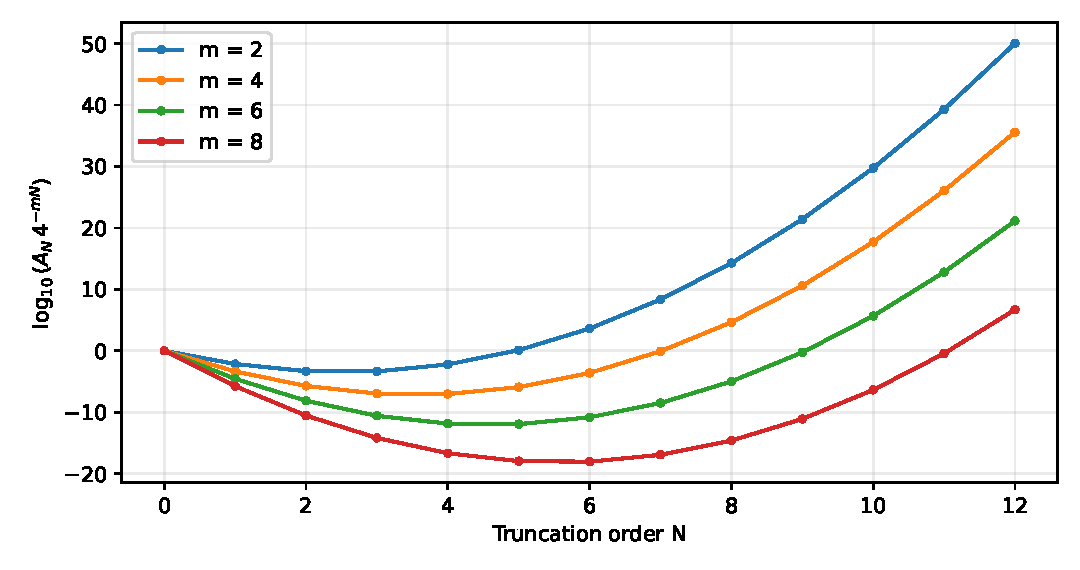
\includegraphics[width=0.93\linewidth]{figures/remainder_bounds.pdf}
 \caption{The proved first-omitted-term bounds $A_N4^{-mN}$.
 Each curve first decreases and then increases. These are values of
 explicit bounds, not measured numerical errors.}
 \label{fig:remainder}
\end{figure}

\section{Gaussian localization of the centered zero strings}
\label{sec:complex-center}
The alternating inequality also controls complex translated
arguments, although the complex remainder no longer has a sign.
This is the quantitative refinement asserted in
\cref{thm:overview}.

\begin{proposition}[Complex centered remainder]
\label{prop:complex-center}
Let $h=2^{-m}$, $s=\sigma+\ii\tau$, and $N\ge0$. Then
\begin{align}
 F_{m,1/2}(s)
 &=C(s)\sum_{r=0}^{N-1}(-1)^rc_r
         2^{2rs+2r^2+r}h^{2r}+R_{m,N}(s),
 \label{eq:center-complex-expansion}\\
 \abs{R_{m,N}(s)}
 &\le c_Nh^{2N}C(\sigma+2N)
 =c_Nh^{2N}2^{2N\sigma+2N^2+N}C(\sigma).
 \label{eq:center-complex-bound}
\end{align}
For $s$ in any fixed compact set, an integer $N=N(m)=m/2+O(1)$
can be chosen so that
\begin{equation}
 \sup_s\abs{R_{m,N(m)}(s)}
 \le \exp[-Lm^2/2+O(m)].
 \label{eq:complex-gaussian-error}
\end{equation}
\end{proposition}
\begin{proof}
Use the Taylor remainder of $\Psi(t)=\E e^{-t^2W}$ for real $t\ge0$:
its absolute value after $N$ even terms is at most $c_Nt^{2N}$.
Insert it into \cref{eq:F-exact}; taking absolute values replaces
$u^{s-1}$ by $u^{\sigma-1}$. This proves the first inequality.
The Mellin shift identity proves the equality.

On a compact set let $\sigma\le b$, and bound $C(\sigma)$ by a
constant. Using $c_N\le BR^{-N}$, the logarithm of the bound is at
most
\[
 2LN^2+\{L(1+2b-2m)-\log R\}N+O(1).
\]
Its minimizing integer is $m/2+O(1)$; substitution gives
\cref{eq:complex-gaussian-error}.
\end{proof}

\begin{theorem}[Centered Gaussian zero clusters]
\label{thm:zero-gaussian}
If $s_0$ is a zero of $C$ of multiplicity $d$, then the $d$ zeros of
$D(\cdot,1/2)$ in the cluster approaching $s_0-m$ satisfy
\begin{equation}
 \abs{s-(s_0-m)}
 \le\exp[-Lm^2/(2d)+O_{s_0}(m)].
 \label{eq:center-zero-bound}
\end{equation}
The same conclusion holds for the corresponding off-axis zeros of
$D(\cdot,1)$.
\end{theorem}
\begin{proof}
Choose a small fixed disk $\mathcal K$ about $s_0$ as in
\cref{thm:zero-strings}. Use the truncation $N(m)$ of
\cref{prop:complex-center}. We must check that the finite
multiplier
\[
 S_m(s)=\sum_{r=0}^{N(m)-1}(-1)^rc_r
        2^{2rs+2r^2+r}h^{2r}
\]
remains nonzero near $s_0$ even though its number of terms grows.
For $1\le r<N(m)$, the bound on the logarithm of the $r$th term is
\[
 2Lr^2+\{L(1+2b-2m)-\log R\}r+\log B.
\]
This convex quadratic decreases until a point $m/2+O(1)$.
On the integer interval from $1$ to $N(m)-1$ its maximum is at an
endpoint. The first endpoint is $-2Lm+O(1)$, while the last is
$-Lm^2/2+O(m)$. Thus
$\sup_{s\in\mathcal K}\abs{S_m(s)-1}=O(m2^{-2m})\to0$.
In particular $\abs{S_m}\ge1/2$ for large $m$.

The local lower bound $\abs{C(s)}\ge g_0\abs{s-s_0}^d$ and
\cref{eq:complex-gaussian-error} now allow Rouch\'e on a circle of
radius $\exp[-Lm^2/(2d)+B_1m]$, for a sufficiently large fixed
$B_1$. The comparison term strictly dominates the remainder.
This gives the asserted $d$ zeros. Identity \cref{eq:half-one}
transfers the statement to $a=1$, since these disks are eventually
disjoint from the imaginary axis.
\end{proof}

The proof is deliberately insensitive to the multiplicity of the
limiting zero. For a simple zero the coefficient $1/d$ is absent;
for a multiple zero it is the natural loss produced by a local
factor $(s-s_0)^d$.

\section{A non-lognormal measure with exact lognormal moments}
\label{sec:moments}

\subsection{Moment equality and genuine distinctness}
Let $V$ be lognormal with
\begin{equation}
 \log V\sim N(L/2,L).
 \label{eq:lognormal}
\end{equation}
Its moments are
$\E V^s=\exp[Ls(s+1)/2]$ for real $s$, and indeed for complex $s$.
By \cref{eq:T-moments},
\begin{equation}
 \E T^n=\E V^n\qquad(n\in\Z).
 \label{eq:integer-twins}
\end{equation}
In logarithmic coordinates, the two densities are
\begin{align}
 f_{\log T}(v)
 &=\frac1{C_0}e^{-v^2/(2L)+v/2}H(v),
 \label{eq:T-log-density}\\
 f_{\log V}(v)
 &=\frac1{\sqrt{2\pi L}}e^{-(v-L/2)^2/(2L)}.
 \label{eq:V-log-density}
\end{align}
Their density ratio is
\begin{equation}
 \frac{\dd\mathbb P_T}{\dd\mathbb P_V}(e^v)
 =\frac{\sqrt{2\pi L}\,e^{L/8}}{C_0}H(v).
 \label{eq:density-ratio}
\end{equation}
It is bounded above and below by positive constants, but it is not
constant. Thus the measures are distinct, despite matching every
positive and negative integer moment.

This is an explicit realization of a classical indeterminate moment
problem. The new role of this particular representing measure is
that it is built from the Thue--Morse product and supplies the
scaling limit for the Dirichlet zero problem. The abstract fact that
lognormal moments do not determine a measure is not new
\cite[Section 9]{AGK}.

\subsection{Size bias and the periodic degree of freedom}
The size-biased law of a positive random variable $T$ with finite
mean is defined by
\[
 \E f(T^*)=\frac{\E[Tf(T)]}{\E T}
\]
for bounded measurable $f$. In the present normalization, $\E T=2$.
A change of variables and \cref{eq:K-dilation} give
\begin{equation}
 T^*\overset{d}=2T.
 \label{eq:size-bias}
\end{equation}
Indeed, the density of $T^*$ is $K(t)/(2C_0)$, and the density of
$2T$ is $K(t/2)/(C_0t)=K(t)/(2C_0)$.

More generally, let $p$ be a bounded $L$-periodic measurable function.
The same Mellin substitution used for \cref{eq:C-step} shows that
\begin{equation}
 \int_0^\infty t^n p(\log t)\mu(\dd t)
 =2^{n(n+1)/2}\int_0^\infty p(\log t)\mu(\dd t)
 \quad(n\in\Z).
 \label{eq:periodic-perturb}
\end{equation}
If $p$ has mean zero under $\mu$, then
$(1+\theta p(\log t))\mu(\dd t)$ is a probability measure with the
same integer moments whenever $\abs\theta\,\|p\|_\infty\le1$.
Choosing a nonconstant $p$ produces infinitely many such measures.

To prove \cref{eq:periodic-perturb} for all integer $n$, define
$C_p(s)=\int t^{s-1}K(t)p(\log t)\dd t$. Boundedness of $p$
permits every integral, and its periodicity gives
$C_p(s+1)=2^{s+1}C_p(s)$ by the same substitution. Iteration at
integer arguments proves the formula, including negative indices.

\subsection{An exact mixture over geometric lattices}
Write every $t>0$ uniquely as $t=v2^k$ with $1\le v<2$ and
$k\in\Z$. Define
\begin{equation}
 \Theta(v)=\sum_{k\in\Z}v^{-k}2^{-k(k-1)/2}.
 \label{eq:Theta}
\end{equation}
The series converges uniformly for $1\le v\le2$. Then
\begin{equation}
 \mu=\int_1^2 \nu_v\,
        \frac{K(v)\Theta(v)}{C_0}\frac{\dd v}{v},
 \label{eq:lattice-mixture}
\end{equation}
where the discrete probability measure $\nu_v$ is supported on
$\{v2^k:k\in\Z\}$ and has weights
\begin{equation}
 \nu_v(\{v2^k\})=
 \frac{v^{-k}2^{-k(k-1)/2}}{\Theta(v)}.
 \label{eq:lattice-weights}
\end{equation}
To verify the identity, split the integral defining $\mu$ into the
intervals $[2^k,2^{k+1})$, substitute $t=2^kv$, and apply
\cref{eq:K-iterate}. This also proves that the mixing density
integrates to one.

Every single $\nu_v$ has the same integer moments:
\begin{equation}
 \int t^n\nu_v(\dd t)=2^{n(n+1)/2}
 \qquad(n\in\Z).
 \label{eq:lattice-moments}
\end{equation}
In fact, shift the summation index by $n$ in the numerator obtained
from \cref{eq:lattice-weights}; completing the exponent gives the
factor $v^{-n}2^{n(n+1)/2}$, which cancels the external $v^n$.
These geometric-lattice moment representatives are classical
Chihara--Leipnik-type laws; see \cite{AGK}. Formula
\cref{eq:lattice-mixture} identifies the particular phase mixture
selected by the Thue--Morse completion.

\section{Exact moment algebra: determinants and orthogonal polynomials}
\label{sec:orthogonal}
The integer moments in \cref{eq:T-moments} make a small amount of
exact algebra available essentially for free. It provides useful
checks on both the normalization and the relation to the
Stieltjes--Wigert moment problem. The algebraic identities themselves
are standard consequences of geometric moments, not independent
priority claims.

\begin{proposition}[Hankel determinant]
\label{prop:determinant}
For every integer $d\ge1$,
\begin{equation}
 \boxed{\displaystyle
 \det\left[2^{(i+j)(i+j+1)/2}\right]_{i,j=0}^{d-1}
 =2^{d^2(d-1)/2}\prod_{k=1}^{d-1}(2^k-1)^{d-k}.}
 \label{eq:hankel-exact}
\end{equation}
\end{proposition}
\begin{proof}
Factor $2^{i(i+1)/2}$ from row $i$ and
$2^{j(j+1)/2}$ from column $j$. The remaining matrix is
$[(2^i)^j]$, whose determinant is the Vandermonde product
$\prod_{0\le i<j<d}(2^j-2^i)$.
In this product factor $2^i$ from each difference. The powers of $2$
from the rows and columns have total exponent
$d(d-1)(d+1)/3$; the extra exponent is
$d(d-1)(d-2)/6$. Their sum is $d^2(d-1)/2$.
A difference $j-i=k$ occurs $d-k$ times, giving the remaining
product.
\end{proof}

Define the Gaussian binomial coefficient at $q=2$ by
\begin{equation}
 \qbinom nk2=\prod_{j=0}^{k-1}
                 \frac{2^{n-j}-1}{2^{j+1}-1}
 \quad(0\le k\le n).
 \label{eq:qbinom}
\end{equation}
Empty products equal one.

\begin{proposition}[Monic orthogonal polynomials]
\label{prop:orthogonal}
The monic degree-$n$ polynomial orthogonal to $1,t,\ldots,t^{n-1}$
under $\mu$ is
\begin{equation}
 \boxed{\displaystyle
 p_n(t)=\sum_{k=0}^n(-1)^{n-k}2^{n(n-k)}\qbinom nk2\,t^k.}
 \label{eq:orthogonal}
\end{equation}
Its squared norm is
\begin{equation}
 \int p_n(t)^2\mu(\dd t)
 =2^{n(3n+1)/2}\prod_{k=1}^n(2^k-1).
 \label{eq:orthogonal-norm}
\end{equation}
The same polynomials and norms apply to every other representing
measure discussed in \cref{sec:moments}.
\end{proposition}
\begin{proof}
For a polynomial $p(t)=\sum_{k=0}^na_kt^k$,
\[
 \int t^jp(t)\mu(\dd t)
 =2^{j(j+1)/2}\sum_{k=0}^n
        a_k2^{k(k+1)/2}(2^j)^k.
\]
Thus orthogonality for $j=0,\ldots,n-1$ is equivalent to the
polynomial identity
\[
 \sum_{k=0}^na_k2^{k(k+1)/2}z^k
 =2^{n(n+1)/2}\prod_{j=0}^{n-1}(z-2^j).
\]
Expanding the product by the finite $q$-binomial identity gives
\cref{eq:orthogonal}. This proves both orthogonality and monicity.
Strict positivity of the Hankel matrices guarantees uniqueness.
The norm is the ratio of the size-$(n+1)$ and size-$n$ Hankel
determinants; substitution of \cref{eq:hankel-exact} gives
\cref{eq:orthogonal-norm}. Alternatively, the same ratio follows
by triangular Gram--Schmidt elimination. Every integral used here
is a polynomial moment, so it is unchanged for any representing
measure with those moments.
\end{proof}

For example,
\[
 p_0(t)=1,\qquad p_1(t)=t-2,\qquad
 p_2(t)=t^2-12t+16.
\]
The norm of $p_1$ is $8-4=4$, agreeing with
\cref{eq:orthogonal-norm}. These low-degree checks are sensitive to
the easily confused alternatives $2^{n(n-1)/2}$ and
$2^{n(n+1)/2}$ in the moment normalization.

\section{Identical asymptotic series, different positive functions}
\label{sec:flat-twins}
The moment interpretation gives a concrete nonuniqueness result for
the all-orders expansion itself. Let $V$ be the lognormal variable
in \cref{eq:lognormal}, independent of the same $W$, and set
\begin{equation}
 \widetilde{\calH}(x)=\E e^{-xV^2W}.
 \label{eq:Htilde}
\end{equation}

\begin{theorem}[A completely monotone beyond-all-orders ambiguity]
\label{thm:flat-twins}
The functions $\calH$ and $\widetilde{\calH}$ are distinct, completely
monotone functions with identical derivatives of every order at
zero. Both satisfy the same alternating bound
\cref{eq:alternating-bound}. Consequently, for every $N\ge0$,
\begin{equation}
 \abs{\calH(x)-\widetilde{\calH}(x)}\le2A_Nx^N
 \qquad(x\ge0).
 \label{eq:flat-twin-bound}
\end{equation}
Optimizing $N$ as in \cref{cor:optimal} gives a logarithmic-Gaussian
upper bound for their difference at small $x$.
\end{theorem}
\begin{proof}
Equality of the integer moments of $T$ and $V$ gives
\[
 \frac{\E(T^2W)^r}{r!}
 =\frac{\E(V^2W)^r}{r!}=A_r
\]
for every integer $r\ge0$. The proof of
\cref{thm:alternating} applies unchanged to both Laplace transforms,
so the derivatives and remainder bounds agree. Subtracting the
same finite polynomial gives \cref{eq:flat-twin-bound}.

Suppose nevertheless that the two functions were identical.
Uniqueness of Laplace transforms for probability measures on
$[0,\infty)$ would imply $T^2W\overset d=V^2W$.
For every real $r>0$, all moments involved are finite and
$\E W^r>0$, so independence permits cancellation:
\[
 \E T^{2r}\,\E W^r=\E V^{2r}\,\E W^r
 \quad\Longrightarrow\quad Q(2r)=1.
\]
The identity theorem would then force $Q\equiv1$, contradicting
\cref{prop:C-Fourier}. Thus the functions are distinct.
\end{proof}

The factor $2$ in \cref{eq:flat-twin-bound} is convenient rather than
optimal: since both functions lie in the same interval between
successive alternating truncations, one can in fact replace it by
$1$. Keeping the weaker bound makes clear that even the triangle
inequality already proves flatness. Either version is enough to
show that every coefficient of the asymptotic expansion can be
known exactly while the function still is not uniquely specified.

This phenomenon is not an arbitrary addition of a small oscillatory
term. Both realizations are positive Laplace transforms and satisfy
all complete-monotonicity inequalities. Thus positivity, smoothness,
and a full asymptotic series still leave a nontrivial ambiguity.
The Thue--Morse product supplies the extra information selecting
$\calH$ rather than its lognormal replacement.

\section{Extension to sparse digit sequences in other integer bases}
\label{sec:bases}
The completion is not restricted to base two. This section records
the extension with enough detail to identify exactly where
integrality of the base is used.

For a real number $b>1$, define
\begin{equation}
 P_b(t)=\prod_{j\ge0}(1-e^{-b^jt}),\qquad
 X_b=\sum_{j\ge1}b^{-j}U_j,\qquad
 \Phi_b(t)=\E e^{-tX_b},\qquad K_b=P_b\Phi_b.
 \label{eq:base-products}
\end{equation}
Now $X_b$ is supported on $[0,1/(b-1)]$ and has mean
$a_b=1/[2(b-1)]$. The same cancellation gives
\begin{equation}
 K_b(bt)=\frac{K_b(t)}t,
 \qquad C_b(s+1)=b^{s+1}C_b(s),
 \label{eq:base-mellin}
\end{equation}
where $C_b(s)=\int_0^\infty t^{s-1}K_b(t)\dd t$.
Thus the normalized measure has moments $b^{n(n+1)/2}$ for every
integer $n$, and the exact logarithmic profile is periodic with
period $\log b$.

When $b\ge2$ is an integer, define $\mathcal S_b$ to be the
nonnegative integers whose base-$b$ digits are all zero or one.
For $n\in\mathcal S_b$, let $w_b(n)$ be the number of nonzero
digits. The product expansion gives
\begin{equation}
 P_b(t)=\sum_{n\in\mathcal S_b}(-1)^{w_b(n)}e^{-nt},
 \label{eq:base-digit-series}
\end{equation}
and hence the sparse signed Dirichlet series
\begin{equation}
 D_b(s,a)=\sum_{n\in\mathcal S_b}
       \frac{(-1)^{w_b(n)}}{(n+a)^s}.
 \label{eq:base-Dirichlet}
\end{equation}
Absolute convergence holds at least in $\Rea s>\log_b2$:
the integers in $\mathcal S_b$ below $b^k$ are exactly $2^k$ in
number, and comparison by base-$b$ blocks proves convergence there.
The Mellin integral continues the series to an entire function just
as before.

\begin{theorem}[Integer-base zero strings]
\label{thm:base-zeros}
For every integer $b\ge2$ and every $a>0$, $D_b(\cdot,a)$ has
infinitely many nonreal zeros in the left half-plane. More precisely,
if $s_0$ is a zero of $C_b$ of multiplicity $d$, the corresponding
clusters approach $s_0-m$ with error smaller than $b^{-Am}$ for
every fixed $A>0$.
At the centered shift $a=a_b$, their error is bounded by
\begin{equation}
 \exp\left[-\frac{\log b}{2d}m^2+O(m)\right].
 \label{eq:base-zero-rate}
\end{equation}
\end{theorem}
\begin{proof}
All the completion and Mellin estimates replace $L$ by $\log b$.
The nonconstancy proof is still valid: because $b^j$ is an integer,
$P_b(x+2\pi\ii)=P_b(x)\to0$, whereas a constant-profile elementary
Gaussian expression would have a nonzero limit there.
The normalized periodic Mellin function is therefore nonconstant,
entire, positive on the real axis, and of order at most two.
Lemma \ref{lem:periodic-zero} supplies a nonreal zero.

Put $B_{b,a}(t)=e^{-at}/\Phi_b(t)$. Since $X_b$ has positive
probability in every neighborhood of zero, the proof of the global
Taylor remainder in \cref{lem:B-global} applies. With $h=b^{-m}$,
exact rescaling gives
\[
 b^{-m(m-1)/2+ms}\Gamma(s-m)D_b(s-m,a)
 =\int_0^\infty u^{s-1}K_b(u)B_{b,a}(hu)\dd u.
\]
At poles of the Gamma factor, the left side is interpreted through
its entire Mellin numerator. The $j$th coefficient is again a multiple of $C_b(s+j)$, and
\cref{eq:base-mellin} factors out $C_b(s)$. The proof of
\cref{thm:zero-strings} now applies verbatim.

For the centered bound,
\[
 B_{b,a_b}(z)=\prod_{j\ge1}
       \frac{z/(2b^j)}{\sinh(z/(2b^j))}
\]
is the Laplace transform in $z^2$ of
\[
 W_b=\sum_{j,n\ge1}\frac{E_{j,n}}{4\pi^2b^{2j}n^2}.
\]
Its first moment-generating pole is at $R_b=4\pi^2b^2$.
Removing the first pole as in \cref{thm:c-asymptotic} bounds its
coefficients by a constant times $R_b^{-r}$. The counterpart of
\cref{eq:center-complex-bound} then has exponent
$2(\log b)N^2-2m(\log b)N+O(N)$.
Optimizing at $N=m/2+O(1)$ and repeating the Rouch\'e argument
proves \cref{eq:base-zero-rate}.
\end{proof}

For noninteger real $b>1$, the positive product, Mellin identity,
and moment construction still hold. The boundary-periodicity step
used to prove nonconstancy does not automatically survive, and
\cref{eq:base-digit-series} is no longer an ordinary integer-indexed
Dirichlet series. We do not silently extend the integer-base zero
claim to that setting.

\section{An explicit Fourier formula for the logarithmic profile}
\label{sec:log-Fourier}
The proofs above need neither zeta values nor an evaluated constant.
For reproducible computation, however, it is useful to make the
profile explicit. Mellin analysis of harmonic sums is a standard
method \cite{FGD}; the calculation is included here to fix every
sign and normalization.

Let $\gamma$ denote Euler's constant and $\gamma_1$ the first
Stieltjes constant in
\begin{equation}
 \zeta(1+z)=\frac1z+\gamma-\gamma_1z+O(z^2).
 \label{eq:stieltjes-convention}
\end{equation}
Define
\begin{equation}
 \chi_k=\frac{2\pi\ii k}{L},\qquad
 c_*=-\frac L{12}-\frac{\pi^2/12-\gamma^2/2-\gamma_1}{L}.
 \label{eq:cstar}
\end{equation}

\begin{proposition}[Exact profile formula]
\label{prop:logH}
For real $v$,
\begin{equation}
 \boxed{\displaystyle
 \log H(v)=c_*-\frac1L\sum_{k\in\Z\setminus\{0\}}
       \Gamma(\chi_k)\zeta(1+\chi_k)e^{-\chi_kv}.}
 \label{eq:logH-Fourier}
\end{equation}
The Fourier series and every fixed derivative converge absolutely.
\end{proposition}
\begin{proof}
For $\Rea z>0$, expanding $\log(1-e^{-t})$ into exponentials and
integrating termwise gives
\[
 \int_0^\infty t^{z-1}\log(1-e^{-t})\dd t
 =-\Gamma(z)\zeta(z+1).
\]
Summing the dyadic dilates, also absolutely for $\Rea z>0$, gives
\begin{equation}
 \log P(t)=-\frac1{2\pi\ii}
 \int_{c-\ii\infty}^{c+\ii\infty}
 \frac{\Gamma(z)\zeta(z+1)}{1-2^{-z}}t^{-z}\dd z,
 \qquad c>0.
 \label{eq:logP-Mellin}
\end{equation}
This Mellin inversion is justified by exponential decay of the
Gamma factor on vertical lines.

Move the line to $\Rea z=-\delta$, with $0<\delta<1$.
The crossed poles are $z=0$ and $z=\chi_k$, $k\ne0$.
One may use horizontal sides at heights
$2\pi(N+1/2)/L$, which stay away from the zeros of the denominator.
Stirling's estimate for $\Gamma$, polynomial bounds for $\zeta$
on this fixed vertical strip, and the bound on the denominator show
that the horizontal integrals tend to zero. On the new vertical
line the integral is $O(t^\delta)$ as $t\downarrow0$.
The residue sum converges absolutely because
$\abs{\Gamma(\chi_k)}$ decays exponentially in $\abs k$.

At a nonzero $\chi_k$, the derivative of $1-2^{-z}$ is $L$, so
its residue contributes
$-\Gamma(\chi_k)\zeta(1+\chi_k)t^{-\chi_k}/L$.
At zero, use
\begin{align*}
 \Gamma(z)\zeta(1+z)
 &=\frac1{z^2}+\left(\frac{\pi^2}{12}
             -\frac{\gamma^2}{2}-\gamma_1\right)+O(z),\\
 \frac1{1-e^{-Lz}}&=\frac1{Lz}+\frac12+\frac{Lz}{12}+O(z^3).
\end{align*}
Multiplication by $t^{-z}$ gives the contribution
\[
 -\frac{(\log t)^2}{2L}+\frac{\log t}{2}+c_*.
\]
Consequently,
\[
 \log P(t)=-\frac{(\log t)^2}{2L}+\frac{\log t}{2}+c_*
 -\frac1L\sum_{k\ne0}\Gamma(\chi_k)\zeta(1+\chi_k)t^{-\chi_k}
 +O(t^\delta).
\]
Since $\log\Phi(t)=O(t)$, comparison with the definition of $H$
gives the claimed Fourier expression plus $O(t^\delta)$ for small
$t$. Finally replace $t$ by $2^{-m}t$. Both the profile and the
Fourier sum are invariant under this substitution, while the error
tends to zero. This turns the asymptotic identity into the exact
formula \cref{eq:logH-Fourier}. Exponential Gamma decay absorbs any
fixed derivative multiplier $\chi_k^r$.
\end{proof}

\begin{figure}[t]
 \centering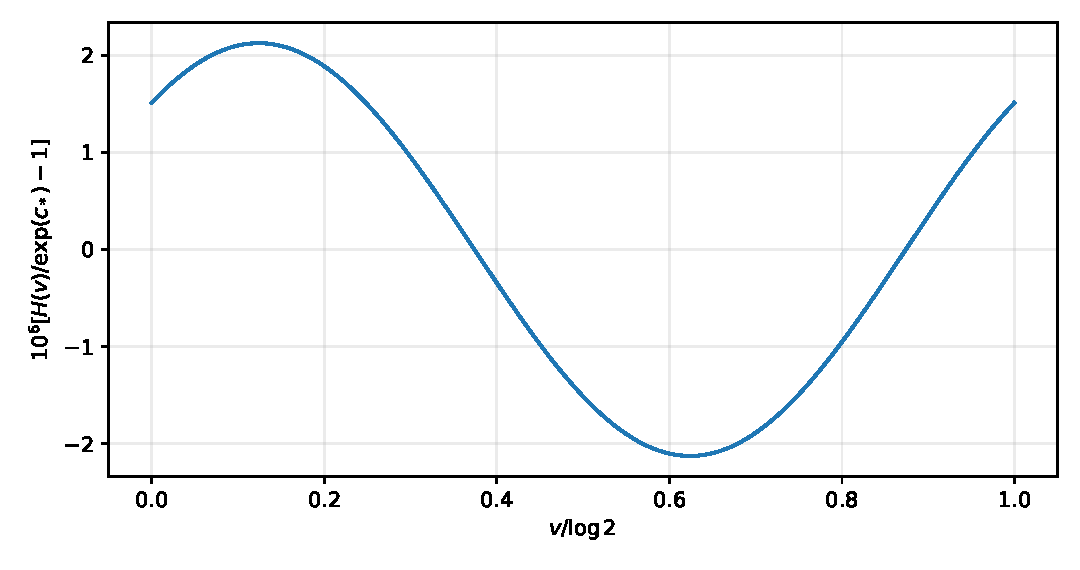
\includegraphics[width=0.93\linewidth]{figures/periodic_profile.pdf}
 \caption{The nonconstant profile $H$ over one logarithmic period.
 The vertical scale is in parts per million relative to $e^{c_*}$.
 This small oscillation is not a negligible detail for the complex
 zero problem.}
 \label{fig:profile}
\end{figure}

The Fourier series for $\log H$ and the Fourier series for $H$
should not be confused. To use \cref{eq:C-Fourier}, first exponentiate
\cref{eq:logH-Fourier}, then calculate the coefficients $h_k$ of the
resulting positive function. Substituting the coefficients of
$\log H$ directly into \cref{eq:C-Fourier} gives an incorrect
normalization and shifts the computed zeros.

\section{Numerical experiments and reproducibility}
\label{sec:numerics}

\subsection{What was computed}
The accompanying script \path{code/verify.py} performs exact rational
coefficient and determinant checks, evaluates $K$ by its products,
evaluates the profile by \cref{eq:logH-Fourier}, and compares direct
Mellin quadrature with the Fourier--Gaussian representation.
It also solves for selected zeros in the normalized variable, using
\cref{eq:F-exact} rather than a very large unnormalized Gamma factor.
The files under \path{data/} contain the numerical outputs.
The completion constant and the displayed limiting zero agree in
separate 60- and 80-digit runs. The script
\path{code/check_original_mellin.py} additionally tests the first
listed Dirichlet zero directly in the original integral
\cref{eq:M-def}, for both $a=1/2$ and $a=1$, without using the
completion to construct its integrand.

These are high-precision floating-point experiments. Their reported
residuals are not interval-arithmetic error certificates. The
existence theorems and the signed remainder bounds are proved
analytically above and do not depend on interpreting a small
floating-point residual as a proof.

The normalizing constant is approximately
\begin{equation}
 C_0=0.7507219804078709592097079140506346947658\ldots.
 \label{eq:C0-numeric}
\end{equation}
One numerically observed simple zero of $C$, chosen in a real
fundamental strip, is
\begin{equation}
 s_0\approx
 0.1240623273169621334141320413937
 +6.7214865334392714744741792585671\,\ii.
 \label{eq:s0-numeric}
\end{equation}
The word ``one'' is intentional: the computation does not establish
that this is the lowest-height nonreal zero, nor that all zeros are
simple. The normalized derivative $Q'(s_0)$ is numerically extremely
close to $2\pi\ii$, consistent with a leading two-term Fourier
balance, but that observation is not used in the proof.

\begin{table}[ht]
\centering\small
\begin{tabular}{@{}rlll@{}}
\toprule
$m$&$\Rea s_m$&$\Ima s_m$&$\abs{s_m-(s_0-m)}$\\
\midrule
4&$-3.8759680374867420$&$6.7214963407429050$&$3.19093\cdot10^{-5}$\\
6&$-5.8759376731062212$&$6.7214865336192914$&$4.59882\cdot10^{-10}$\\
8&$-7.8759376726830382$&$6.7214865334392717$&$4.19307\cdot10^{-16}$\\
\bottomrule
\end{tabular}
\caption{Numerical zeros of $D(s,1/2)$ and, by
\cref{eq:half-one}, of $D(s,1)$. The distances refer to the
higher-precision value of $s_0$ stored in the data file.}
\label{tab:zeros}
\end{table}

The centered slope ratios provide an independent positive-axis
check:
\begin{table}[ht]
\centering
\begin{tabular}{@{}rl@{}}
\toprule
$m$&$Z_m(1/2)/(C_0\,2^{m(m-1)/2})$\\
\midrule
0&$0.9233074275823854568421676411$\\
2&$0.9934028797641805193051831301$\\
4&$0.9995677618356360314893011938$\\
6&$0.9999728805385416834067380219$\\
8&$0.9999983046075012694941809752$\\
\bottomrule
\end{tabular}
\caption{Direct Mellin quadrature of the exact samples
$\calH(4^{-m})$. The script checks the signed inequalities for
truncation orders one through seven.}
\label{tab:ratios}
\end{table}

\subsection{Stable product evaluation}
For positive $t$, compute $\log P(t)$ as a sum of
$\log(-\operatorname{expm1}(-2^jt))$ rather than by subtracting nearly
equal floating-point numbers. Its omitted large-scale terms decrease
doubly exponentially.

For $\Phi(t)$, first apply enough halvings that the remaining argument
$v$ lies in $(0,1]$. Multiply the finitely many removed factors
exactly at working precision. The infinite remaining tail is then
computed from
\begin{equation}
 \log\Phi(v)=-\frac v2+
 \sum_{r\ge1}\frac{B_{2r}v^{2r}}{2r(2r)!(2^{2r}-1)}.
 \label{eq:Phi-numeric}
\end{equation}
This avoids multiplying hundreds of factors close to one. Both the
product route and the Fourier route are retained in the script so
that they can cross-check one another.

For the zeta values in \cref{eq:logH-Fourier}, the points
$1+2\pi\ii k/L$ are exact dyadic resonances. An implementation using
$\zeta(s)=\eta(s)/(1-2^{1-s})$ naively can lose precision there,
since both numerator and denominator vanish. The supplied code
explicitly requests Euler--Maclaurin evaluation of $\zeta$.
In the tested \texttt{mpmath} environment this avoided a visible
loss of accuracy in the profile. This is an implementation detail,
not a mathematical singularity of $\zeta$ at these points.

\subsection{Why the Mellin quadrature is manageable}
In logarithmic coordinates, the integrand for $C$ is a Gaussian
multiplied by a bounded periodic function and $e^{sv}$.
For a fixed complex $s$, the center of its absolute Gaussian
majorant is $L(\Rea s+1/2)$. The code chooses its finite integration
interval using that center and the requested precision.
At the centered shift, $0<\Psi(2^{-m}e^v)\le1$, so the same
Gaussian tail estimate also controls $F_{m,1/2}$.

The finite interval and quadrature discretization are not
interval-certified in this implementation. Repeating at increased
precision and comparing two analytic representations gives a strong
consistency check, while the proofs supply the logical foundation.
The exact rational calculations, by contrast, are exact: the
coefficient formulas and Hankel determinants are evaluated with
\texttt{SymPy} rationals and integers.

\subsection{Reproduction commands}
From the article directory, a typical run is
\begin{lstlisting}
python -m pip install -r code/requirements.txt
python code/verify.py --dps 60 --roots --figures
python code/verify.py --dps 80
pdflatex -interaction=nonstopmode Thue_Morse_Dyadic_Completion.tex
pdflatex -interaction=nonstopmode Thue_Morse_Dyadic_Completion.tex
\end{lstlisting}
The PDF figures are included in the archive, so compiling the article
does not require running Python first. The exact versions used for
the stored computation are recorded in \path{code/requirements.txt}.
No network requests are made by the verification script.

\section{Relation to the atlas and a formalization route}
\label{sec:audit}

\subsection{Repository audit and limits of the novelty claim}
The requested atlas source was inspected through the repository's
native file interface. The retrieved source blob had SHA
\begin{center}\small\path{7be75f3bc86f9c6712eec6d7550eaea53716434a}.\end{center}
The document's front matter identifies it as consolidated on
28 August 2026. The comparison concentrated on the Laplace-product,
boundary-flatness, Mellin--Dirichlet, and master-product sections,
with targeted repository searches for related moment and zero
material. This was not a line-by-line audit of every file in the
large surrounding research tree.

The atlas already establishes the positive product, effective
flatness, entire continuation, zeros at nonpositive integers, the
dyadic parameter equation, and the bridge from $D'(0,a)$ to
Thue--Morse infinite products. These are inputs or short consequences
in the present article, not asserted additions to the atlas.
The surrounding corpus also contains spectral moment constructions
related to Stieltjes--Wigert measures and reciprocal-transform
polynomials. Accordingly, the existence of such general themes is
not presented as novel either.

The specific extension developed here is the completion $P\Phi$
with its exact Mellin shift, its nonconstant entire periodic factor,
the all-orders factorization of the translated Dirichlet family,
and the resulting zero strings. The centered exponential-mixture
representation then upgrades a formal coefficient calculation to
a signed, globally valid error theorem and an optimized bound.
Those are the statements whose proofs should be compared against
future literature findings.

The public literature checked included the original Dirichlet-series
work and later automatic-series framework \cite{AC,AMP}, Allouche's
zero question \cite{AlloucheQuestions}, T\'oth's related Dirichlet
identities \cite{Toth}, Fabius-function treatments
\cite{Arias,Haugland}, and the probability survey \cite{AGK}.
The relevant Alkauskas preprint was identifiable bibliographically
but its full text was not accessible during this investigation.
Absence of a matching result from these searches is not proof of
priority.

\subsection{A proof-oriented dependency chain}
A formal development can be organized into four layers, without
requiring the numerical Fourier formula for the principal theorem.
First prove positivity and normal convergence of $P$ and $\Phi$,
then their two scaling equations. This yields $K(2t)=K(t)/t$ and
positive upper and lower bounds for its logarithmic profile.

Next establish the Gaussian domination needed for the entire Mellin
transform and its derivatives. The Mellin shift, periodicity of $Q$,
and the boundary contradiction proving nonconstancy can then be
formalized independently of coefficient calculations. The zero-free
finite-order lemma and a version of Rouch\'e with multiplicities
complete the complex-analytic layer.

The asymptotic layer consists of the positive-axis global Taylor
bound for $B_a$ and the exact change of variables in
\cref{eq:F-exact}. Once these are available, the all-orders
factorization is a finite-sum integration lemma, and the
supergeometric zero-cluster theorem is a uniform remainder estimate
followed by Rouch\'e.

Finally, the centered layer adds Euler's $\sinh$ product, the
positive exponential-sum law $W$, and an integral Taylor remainder.
It supplies the signed bounds, the coefficient-pole estimate, and
the Gaussian refinement. The finite Bell-polynomial formula and the
Hankel determinant can be developed in a separate exact algebra
module.

The existing atlas names modules such as
\path{ThueMorseBoundaryFlatness.lean} and
\path{ThueMorseEntireContinuation.lean} for relevant background.
No new Lean file is supplied here, and no theorem in this extension
is claimed to have been machine-checked. The dependency chain is a
technical implementation guide, not a formalization status claim.

\section{Further questions suggested by the proved results}
\label{sec:questions}
The following questions concern refinements not needed for any
preceding theorem.

\begin{question}[Zeros in a fundamental strip]
Can the nonreal zeros of $Q$ in $0\le\Rea s<1$ be counted and
localized effectively as their imaginary parts grow? Are they all
simple?
\end{question}
The Fourier--Gaussian representation is a natural starting point.
At increasing height, different Fourier harmonics compete. A
rigorous two-term dominance argument on suitable contours could
produce explicit zero enclosures, but the present computation is
not a proof of such a global pattern.

\begin{question}[Leading exponentially small displacement]
For a simple zero $s_0$ of $C$, determine an asymptotic equivalent,
not just an upper bound, for $s_m-(s_0-m)$ at the centered shift.
\end{question}
All algebraic powers of $2^{-m}$ vanish from the displacement.
The nearest poles of $\Psi$ and the logarithmic-Gaussian saddle
suggest a more detailed exponentially small analysis. Such an
analysis must retain the phase information in $H$; replacing the
completion by its lognormal twin would erase the zeros of the
limiting periodic factor.

\begin{question}[Growing-height zero windows]
How far may $\abs{\Ima s}$ grow with $m$ while the translated
asymptotic expansion remains useful for zero localization?
\end{question}
The remainder bound in \cref{eq:F-remainder-explicit} depends on
$\Rea s$ but not directly on $\Ima s$. The difficulty is instead a
lower bound for $C(s)$ on the contours used by Rouch\'e. Thus this
question couples growth of the periodic entire factor to the
geometry of its zeros.

\begin{question}[Noninteger dilation]
For every real $b>1$, is the logarithmic profile of $K_b$ nonconstant?
What replaces the integer-frequency boundary argument when $b$ is
not an integer?
\end{question}
An affirmative answer would extend the Mellin zero mechanism to a
continuous family of generalized exponential sums. The exact
completion and moment identities already hold; the missing step in
the proof given here is the nonconstancy argument in that greater
generality.

\subsection*{Closing perspective}
The most useful organizing fact is a cancellation between an
expanding product and a contracting one. The Thue--Morse product
alone carries a complicated dyadic scale dependence; the
uniform-convolution transform removes its nonmonomial factor.
The resulting exact law $K(2t)=K(t)/t$ simultaneously explains
lognormal integer moments, the negative-argument scale of the
Dirichlet continuation, the universal factor in every asymptotic
coefficient, and the occurrence of nonreal zero strings.
At the half-shift, symmetry supplies an additional positive
Laplace representation and converts the expansion into certified
inequalities. The log-periodic information is small on the real
axis, but it is precisely the information that survives beyond all
orders and controls the complex zeros.

\appendix
\section{Coefficient register and normalization checks}
\label{app:coefficients}
The first six coefficients in the centered expansion are
\begin{center}\small
\begin{tabular}{@{}cl@{}}
\toprule
$r$&$A_r$ in $\calH(x)\sim\sum_{r\ge0}(-1)^rA_rx^r$\\
\midrule
0&$1$\\[2pt]
1&$1/9$\\[2pt]
2&$248/2025$\\[2pt]
3&$4806656/2679075$\\[2pt]
4&$3993751257088/10247461875$\\[2pt]
5&$454890030220640780288/345944065438125$\\
\bottomrule
\end{tabular}
\end{center}
All are obtained by the finite formula \cref{eq:c-finite} followed
by multiplication by $2^{2r^2+r}$. Their rapid growth is predicted
by \cref{thm:c-asymptotic}; it is not numerical instability.

The following identities are convenient independent checks:
\begin{align*}
 &\Phi(0)=1,\quad \Phi'(0)=-\tfrac12,\quad
    [z^2]\log\Phi(z)=\tfrac1{72},\\
 &K(2t)t=K(t),\quad C(1)=2C_0,\quad C(-1)=C_0,\\
 &\E T^2=8,\quad \E W=\tfrac1{72},\quad
    \E(T^2W)=\tfrac19,\\
 &Z_m(1/2)=C_0\,2^{m(m-1)/2}\calH(4^{-m}),\\
 &D(s,1/2)=(1+2^s)D(s,1).
\end{align*}
There is also an exact normalization check at $m=0$:
\[
 Z_0(1/2)=L,\qquad Z_0(1)=L/2,\qquad C_0\calH(1)=L.
\]
Indeed, $P(2u)-P(u)=e^{-u}P(2u)$, so substitution $t=2u$ gives
\[
 M(0,1/2)=\int_0^\infty\frac{P(2u)-P(u)}u\dd u=L.
\]
To justify the last equality without splitting divergent integrals,
integrate first over $[\epsilon,R]$. The difference is
$\int_R^{2R}P(u)\dd u/u-\int_\epsilon^{2\epsilon}P(u)\dd u/u$;
use $P(\infty)=1$ and $P(0)=0$. Differentiating
\cref{eq:half-one} at zero gives the value at $a=1$.
These are classical product-normalization consequences, recorded
here as checks rather than new evaluations.

A sign error in the logarithmic centering changes the odd
coefficients; a missing factor of $2$ in the Mellin scaling changes
the moment law; and confusing $\Psi(z)$ with $\Psi(\sqrt z)$ changes
the optimal truncation scale. Each of these errors is detected by
at least one of the checks above.

\section{A direct nonrecursive formula for every asymptotic coefficient}
For readers wishing to implement the general-shift expansion without
Bell-polynomial conventions, define $b=1/2-a$ and
\[
 d_r=-\frac{B_{2r}}{2r(2r)!(2^{2r}-1)}.
\]
Then its coefficient $\alpha_j(a)=2^{j(j+1)/2}\beta_j(a)$ is
\begin{equation}
 \boxed{\displaystyle
 \alpha_j(a)=2^{j(j+1)/2}
 \sum_{\substack{n_0,n_1,\ldots,n_{\lfloor j/2\rfloor}\ge0\\
 n_0+2n_1+4n_2+\cdots+2\lfloor j/2\rfloor n_{\lfloor j/2\rfloor}=j}}
 \frac{b^{n_0}}{n_0!}
 \prod_{r=1}^{\lfloor j/2\rfloor}\frac{d_r^{n_r}}{n_r!}.}
 \label{eq:alpha-final}
\end{equation}
The sum is finite. At $b=0$, only even $j=2r$ survive, and
$\alpha_{2r}(1/2)=(-1)^rA_r$. For the complex translated expansion,
simply multiply its $j$th coefficient by $2^{js}$ before multiplying
by $C(s)$. Thus a single finite coefficient formula covers both the
real-zero slopes and the complex zero-string expansion.

\clearpage
\begingroup\small
\begin{thebibliography}{99}
\bibitem{atlas}
Vladimir Reshetnikov's \texttt{ProveIt} repository,
\emph{The Thue--Morse Sequence: Formula Atlas and Fabius--Rvachev
Frontier Results}, consolidated 28 August 2026; source inspected
4 September 2026.\par
\sourcepath\par
\url{https://github.com/VladimirReshetnikov/ProveIt/tree/main/Analysis/FabiusFunction/docs/semi-formalized-research-frontiers/drafts/thue-morse/Thue_Morse_Atlas_and_Frontiers}.

\bibitem{AC}
J.-P. Allouche and H. Cohen,
\emph{Dirichlet series and curious infinite products},
Bulletin of the London Mathematical Society \textbf{17} (1985),
531--538. \url{https://doi.org/10.1112/blms/17.6.531}.

\bibitem{AMP}
J.-P. Allouche, M. Mend\`es France, and J. Peyri\`ere,
\emph{Automatic Dirichlet series},
Journal of Number Theory \textbf{81} (2000), 359--373.
\url{https://doi.org/10.1006/jnth.1999.2487}.

\bibitem{AlloucheQuestions}
J.-P. Allouche,
\emph{Thue, Combinatorics on words, and conjectures inspired by the
Thue--Morse sequence}, arXiv:1401.3727, version 2 (2014),
Section 3.2. \url{https://arxiv.org/abs/1401.3727}.

\bibitem{Toth}
L. T\'oth,
\emph{Linear combinations of Dirichlet series associated with the
Thue--Morse sequence}, Integers \textbf{22} (2022), A98.
\url{https://arxiv.org/abs/2211.13570}.

\bibitem{Alkauskas}
G. Alkauskas,
\emph{Dirichlet series, associated with Thue--Morse sequence},
Vilnius University, Department of Mathematics, preprint 2001-15
(2001). Bibliographical reference only: the full text was not
retrieved in this investigation. Author's publication list:
\url{https://web.vu.lt/mif/g.alkauskas/math/index.html}.

\bibitem{AGK}
R. Arratia, L. Goldstein, and F. Kochman,
\emph{Size bias for one and all}, Probability Surveys \textbf{16}
(2019), 1--61, especially Section 9.
\url{https://doi.org/10.1214/13-PS221};
\url{https://arxiv.org/abs/1308.2729}.

\bibitem{FGD}
P. Flajolet, X. Gourdon, and P. Dumas,
\emph{Mellin transforms and asymptotics: Harmonic sums},
Theoretical Computer Science \textbf{144} (1995), 3--58.
\url{https://doi.org/10.1016/0304-3975(95)00002-E}.

\bibitem{Arias}
J. Arias de Reyna,
\emph{Arithmetic of the Fabius function}, Integers \textbf{18}
(2018), A51. \url{https://math.colgate.edu/~integers/s51/s51.pdf}.

\bibitem{Haugland}
J. K. Haugland,
\emph{Evaluating the Fabius function}, arXiv:1609.07999 (2016), version 2 (2020).
\url{https://arxiv.org/abs/1609.07999}.
\end{thebibliography}
\endgroup
\end{document}
